%%%%%%%%%%%%%%%%%%%%%%%%%%%%%%%%%%%%%%%%%%%%%%%%%%%%%%%%%%%%%%%%%%%%%%%%%%%%%%%%
%2345678901234567890123456789012345678901234567890123456789012345678901234567890
%        1         2         3         4         5         6         7         8

%\documentclass[letterpaper, 10 pt, conference]{ieeeconf} % Comment this line out
                                                          % if you need a4paper
%\documentclass[a4paper, 10pt, conference]{ieeeconf}      % Use this line for a4
\documentclass[conf]{ieeeconf}                            % paper

\IEEEoverridecommandlockouts                              % This command is only
                                                          % needed if you want to
                                                          % use the \thanks command
\overrideIEEEmargins
% See the \addtolength command later in the file to balance the column lengths
% on the last page of the document

% The following packages can be found on http:\\www.ctan.org
\usepackage{graphics} % for pdf, bitmapped graphics files
\usepackage{epsfig}   % for postscript graphics files
\usepackage{mathptmx} % assumes new font selection scheme installed
\usepackage{times}    % assumes new font selection scheme installed
\usepackage{amsmath}  % assumes amsmath package installed
\usepackage{amssymb}  % assumes amsmath package installed
%\usepackage[pdftex]{graphicx}
\hyphenation{op-tical net-works semi-conduc-tor}

%%%%%%%%%%%%%%%%%%%%%%%%%%%%%%%%%%%%%%%%%%%%%%%%%%%%%%%%%%%%%%%%%%%%%%%%%%%%%%%%



\begin{document}
\title{\LARGE \bf Humanoid Pitching at a Major League Baseball Game: Challenges, Approach, Implementation and Lessons Learned }

\author{ \parbox{3 in}{\centering Daniel M. Lofaro \\
%         \thanks{*Use the $\backslash$thanks command to put information here}\\
         Electrical and Computer Engineering \\
         Drexel University\\
         Philadelphia, PA, USA\\
         {\tt\small dan@danLofaro.com}}
         \hspace*{ 0.5 in}
         \parbox{3 in}{ \centering Paul Oh \\
%         \thanks{**The footnote marks may be inserted manually}\\
         Mechanical Engineering \\
         Drexel University\\
				 Philadelphia, PA, USA\\
         {\tt\small paul@coe.drexel.edu}}
         }
         
   

% make the title area
\maketitle


\begin{abstract}
%\boldmath
Three different approaches of having a full-size humanoid throw the first pitch at a Major League Baseball game are tested and implemented.  
The approaches include kinematic mapping using a motion capture system to capture a human's throwing motion then mapping that to a full-size humanoid.  
The second method is a fully automated approach that uses the sparse reachable map to provide viable full body throwing trajectories to provide the end effector with the desired velocity.  
The third approach borrows from the animation industry.  
The key-frames of the desired trajectory are constructed by hand.  
The time between each key-frame is defined by the user.  
Interpolation methods are used to smoothly move between key frames while limiting the jerk.  
Each method is analyzed and tested in simulation and on physical hardware.  
The full-size humanoid used is the Hubo series robot.  
Based on the latter tests one method was chosen to successfully throw the ceremonial first pitch at a Major League Baseball game in April 2012.
\end{abstract}
% IEEEtran.cls defaults to using nonbold math in the Abstract.
% This preserves the distinction between vectors and scalars. However,
% if the conference you are submitting to favors bold math in the abstract,
% then you can use LaTeX's standard command \boldmath at the very start
% of the abstract to achieve this. Many IEEE journals/conferences frown on
% math in the abstract anyway.

% no keywords




% For peer review papers, you can put extra information on the cover
% page as needed:
% \ifCLASSOPTIONpeerreview
% \begin{center} \bfseries EDICS Category: 3-BBND \end{center}
% \fi
%
% For peerreview papers, this IEEEtran command inserts a page break and
% creates the second title. It will be ignored for other modes.
\IEEEpeerreviewmaketitle

\section{Introduction}
% no \IEEEPARstart
In early February 2012 the director of the Philadelphia Science Festival asked the Drexel Autonomous Systems Lab (DASL)\footnote{Drexel Autonomous Systems Lab: http://dasl.mem.drexel.edu}\label{foot:dasl} if they could have their full-size humanoid Jaemi Hubo throw the ceremonial first pitch at the second annual \textit{Science Night at the Ballpark}.  
On April 28th, 2012 Hubo successfully threw the first pitch at the Philadelphia Phillies vs. Chicago Cubs game in front, see Fig.~\ref{fig:hubo-throw}.
There were 45,196 fans at the game and thousands more were watching it on telivision acording to USA Today.

\begin{figure}[t]
  \centering
\includegraphics[width=1.0\columnwidth]{./pix/hubo-pitch.png}
  \caption{Hubo successfully throwing the first pitch at the second annual Philadelphia Science Festival event Science Night at the Ball Park on April 28th, 2012.  The game was between the Philadelphia Phillies and the Chicago Cubs and played at the Major League Baseball stadium Citizens Bank Park.  The Phillies won 5-2.  Video of the pitch can be found at http://danlofaro.com/Humanoids2012/\#pitch}
  \label{fig:hubo-throw}
\end{figure}


%The PhillieBot\footnote{PhillieBot Video: http://youtu.be/ShId-vZ-ZEY} made by the GRASP Lab at the University of Pennsylvania was the robot that threw the first pitch at the first annual Philadelphia Science Festival \textit{Science Night at the Ballpark} in 2011.  

Hubo was the first full-size humanoid to throw the inaugural pitch at a Major League Baseball game.  
This task poses challenges in the area of fully-body locomotion, coordination and stabilization that must be addressed.
This paper describes how the latter was done via the analyses/tests of three different approaches and the resulting final design.
Section~\ref{sec:background} gives a brief introduction to work already done in the field as well as states the requirements for the pitch.
Section~\ref{sec:methodology} describes the three different methods tested where:
Section~\ref{sec:sec:balance} discusses the balancing methods and criteria used.
Section~\ref{sec:sec:mocap} describes the human-robot kinematic mapping approach that uses a motion capture system to capture a human's throwing motion then mapping that to a full-size humanoid.  
Section~\ref{sec:sec:srm} describes a fully automated approach that uses the sparse reachable map (SRM) to provide viable full body throwing trajectories with the desired end effector velocity\cite{dlofaro-srm}.
Section~\ref{sec:sec:keyframe} describes the final method explored which is based on key-frame trajectories.
Section~\ref{sec:comparison} compares the tests and analyses of each of the methods.
Section~\ref{sec:finalDesign} describes the finial design in detail and the modifications needed to make the robot's pitch reliable.
Finally Section~\ref{sec:conclusion} gives final thoughts and possible improvements for future years.


%% remember robust and to say that you learned from upenns mistakes etc.
\section{Background and Objectives}\label{sec:background}

The objective is to have our humanoid Jaemi Hubo throw a regulation Major League Baseball ball from the pitchers mound across home plate, a distance of 60.5 feet (18.4 m).  
The regulation Major League Baseball ball has a circumference between $9 - 9\frac{1}{4}$ inches (229-235 mm) and weights $5-5\frac{1}{4}$ ounces (142-149 g)\cite{mlbrules}.  
When children are asked to throw the first pitch it is typical for them to stand halfway between the pitchers mound and home plate.
The robot used to throw the pitch, Jaemi Hubo, stands 130 cm tall, the average height of a ten year old child.
To properly fit the stature of the robot the pitch will be given from half the regulation distance.
Using the well known projectile motion formulation it is determined that the robot must have an end effector velocity of 9.47 $\frac{m}{s}$ at $45^o$ when it releases the ball in order for it to cross the plate.
%When Hubo moved to and from the field Jaemi would 

Along with the technical challenges the primary objective sought to anthropomorphize robotic pitching.  
As such Jaemi Hubo was outfitted with a uniform shirt and cap.
In addition Jaemi gestures the crowd by waving its hand when entering and exiting the field.
Thus, beyond simply pitching, the challenge was to engage the audience hence the \textit{Science Night at the Ballpark}.


%is the highly articulated 40 degree of freedom (DOF) adult-size humanoid 


%The pitch is in front of an audience of over 30,000 with thousands more watching on television.
%Failure to successfully throw the ball is not an option.
%Learning from past attempts of dexterous robots under throwing the ball 

Completing the technical objective with a humanoid consists of two major parts: 1) end-effector velocity control and 2) balance/stabilization. 
There are many examples of throwing/pitching machines made by commercial companies such as Louisville Slugger$^{TM}$, Jugs$^{TM}$, and Atec$^{TM}$ to name a few.  
%These devices typically contain one to two fly wheels that the ball travels through in order to be launched or a spring loaded arm that is compressed and released.
%Robots designed for throwing come in many shapes and sizes depending on the objective.  
%2-DOF mechanisms are able to throw in $R^3$ space with the correct kinematic structure.  
%Visual feedback was used in the basketball throwing robot ($\leq 7$ DOF) by Hu et al.~\cite{5649335} achieving an accuracy of 99\% at distances $\leq$ 3 m.  
%This robot was fixed to the ground to guarantee stability.
The PhillieBot\footnote{PhillieBot Video: http://youtu.be/ShId-vZ-ZEY} made by the GRASP Lab at the University of Pennsylvania was the robot that threw the first pitch at the first annual Philadelphia Science Festival \textit{Science Night at the Ballpark} in 2011.  
The PhillieBot consisted of a $\leq 7$ DOF arm with a pneumatic wrist actuator to increase end-effector velocity at the release point.  
The arm was attached to a wheeled mobile platform.
All of these robots/devices are well planted to the ground/base to ensure stability.
None of the latter robots is are anthropomorphic thus limiting their audience engagement.

\begin{figure*}[t]
  \centering
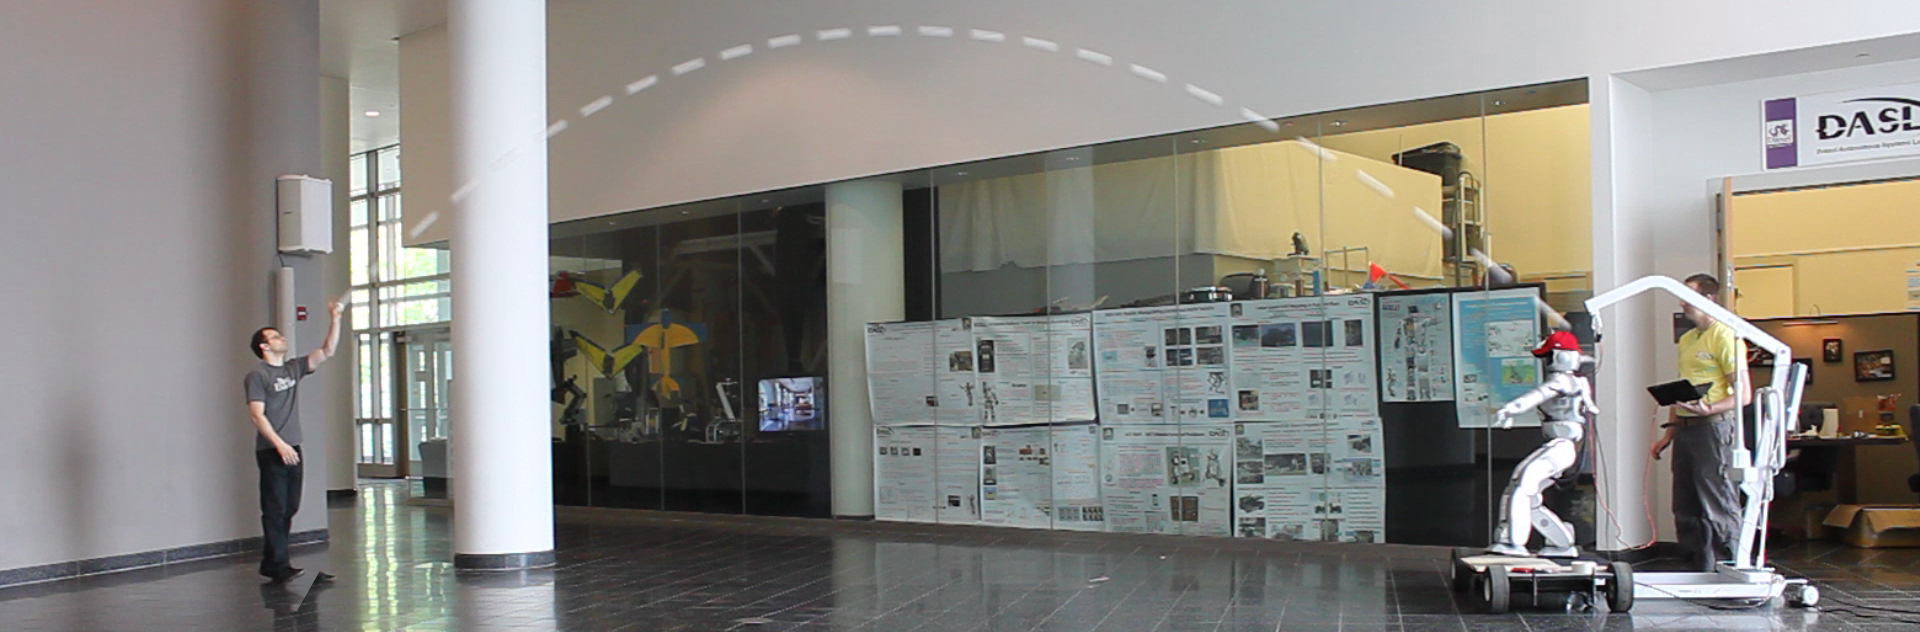
\includegraphics[width=1.0\textwidth]{./pix/preThrow2.png}
  \caption{Frame overlay of the Hubo throwing overhand a distance of 10 m (32.8 feet) with a release angle of 40$^o$ and a tip speed of 10 $\frac{m}{s}$.  Captured at 20 fps with a shutter speed of 1/30 sec.  Each of the white dashes of in the image is the actual baseball as picked up by the video camera.}
  \label{fig:hubo-throw-test}
\end{figure*}


Kim et al. \cite{5686315,JooH2011438} takes the research to the next level with finding optimal overhand and sidearm throwing motions for a high degree of freedom humanoid computer model.  
The model consists of 55-DOF and is not fixed to mechanical ground or a massive base.  
Motor torques are then calculated to create both sidearm and overhand throws that continuously satisfies the zero-moment-point stability criteria~\cite{4309277}.  

\begin{figure}[t]
  \centering
\includegraphics[width=1.0\columnwidth]{./pix/huboExample.png}
  \caption{Jaemi Hubo is a 130 cm tall 37 kg 40-DOF highly articulated, high-gain position controlled, full-size humanoid.}
  \label{fig:huboFig}
\end{figure}


%% needs to be modified
The highly articulated 40-DOF full-size humanoid Jaemi Hubo (Fig.~\ref{fig:huboFig}) is the platform focused on in this work.  Jaemi Hubo is a high-gain, position-controlled biped humanoid weighing 37 kg and standing 130 cm tall.  It is designed and made by Dr. Jun-Ho Oh director of the Hubo Lab at the Korean Advanced Institute of Science and Technology (KAIST).  Jaemi has been located at the Drexel Autonomous Systems Lab (DASL) at Drexel University since the Fall of 2008.  DASL has extensive experience with the Jaemi Hubo KHR-4 platform in key areas needed to complete this work.  Balancing was explored when developing a real-time zero moment point (ZMP) preview control system for stable walking~\cite{5686276}.  A full-scale safe testing environment designed for experiments with Jaemi Hubo was created using DASL's Systems Integrated Sensor Test Rig (SISTR)~\cite{5686325}.  Additionally all algorithms are able to be tested on miniature and virtual versions of Jaemi Hubo prior to testing on the full-size humanoid through the creation of a surrogate testing platform for humanoids~\cite{5379582}.



%Such a mechanism can choose its release point or its end-effector velocity but not both.  
%Mechanisms containing 3 or more DOF with the correct kinematic structure are able to throw in $R^3$ and choose both the release point and the end-effector velocity simultaneously.

% need to modify
%Low degree of freedom throwing machines/robots are common.  Typical throwing robots have between one and three degrees of freedom (DOF)~\cite{509405, Lynch97dynamicnonprehensile, 5152525, 509335, springerlink:10.1007/s10015-006-0401-0}.  All of these mechanisms are limited to throwing in a plane.   Sentoo et al.~\cite{4651142} achieved an end-effector velocity of 6.0 m/s and can throw in $R^3$ space using it's Barret Technology Inc 4-DOF arm with a $360^o$ rotation base yaw actuator.  These low degree of freedom throwing robots are either physically attached/planted to the mechanical ground or have a base that is significantly more massive then the arm. 

%Haddadin et al.\cite{6094757} used their 7-DOF arm and a 6-DOF force torque sensor with standard feedback methods to dribble a basket ball.  In addition Zhikun et al.~\cite{6094892} used reinforcement learning to teach their 7-DOF planted robot arm to play ping-pong.  Likewise Schaal et al.~\cite{schaal01/BIRG} taught their high degree of freedom (30-DOF) humanoid robot to hit a tennis ball using on-line special statistical learning methods. 
\section{Methodology}\label{sec:methodology}
\subsection{Balance and Stability}\label{sec:sec:balance}
Each of the methods used have to be stable through the motion in order for the system to be stable (i.e. not to fall down).  
The well known zero-moment-point (ZMP) criteria is what each method must adhere to in order to stay statically stable\cite{Vukobratovic19721}.  
To handle perturbation an active balance controller was added.  
The active balance controller is applied on top of the pre-defined trajectories.  
Hubo is modeled as a single inverted pendulum with the center of mass (COM) located at length $L$ from the ankle.  
The compliance of the robot is composed of a spring $K$ and a damper $C$, see Fig.~\ref{fig:invPen}.  
An IMU located at the COM gives the measured orientation.

\begin{figure}[t]
  \centering
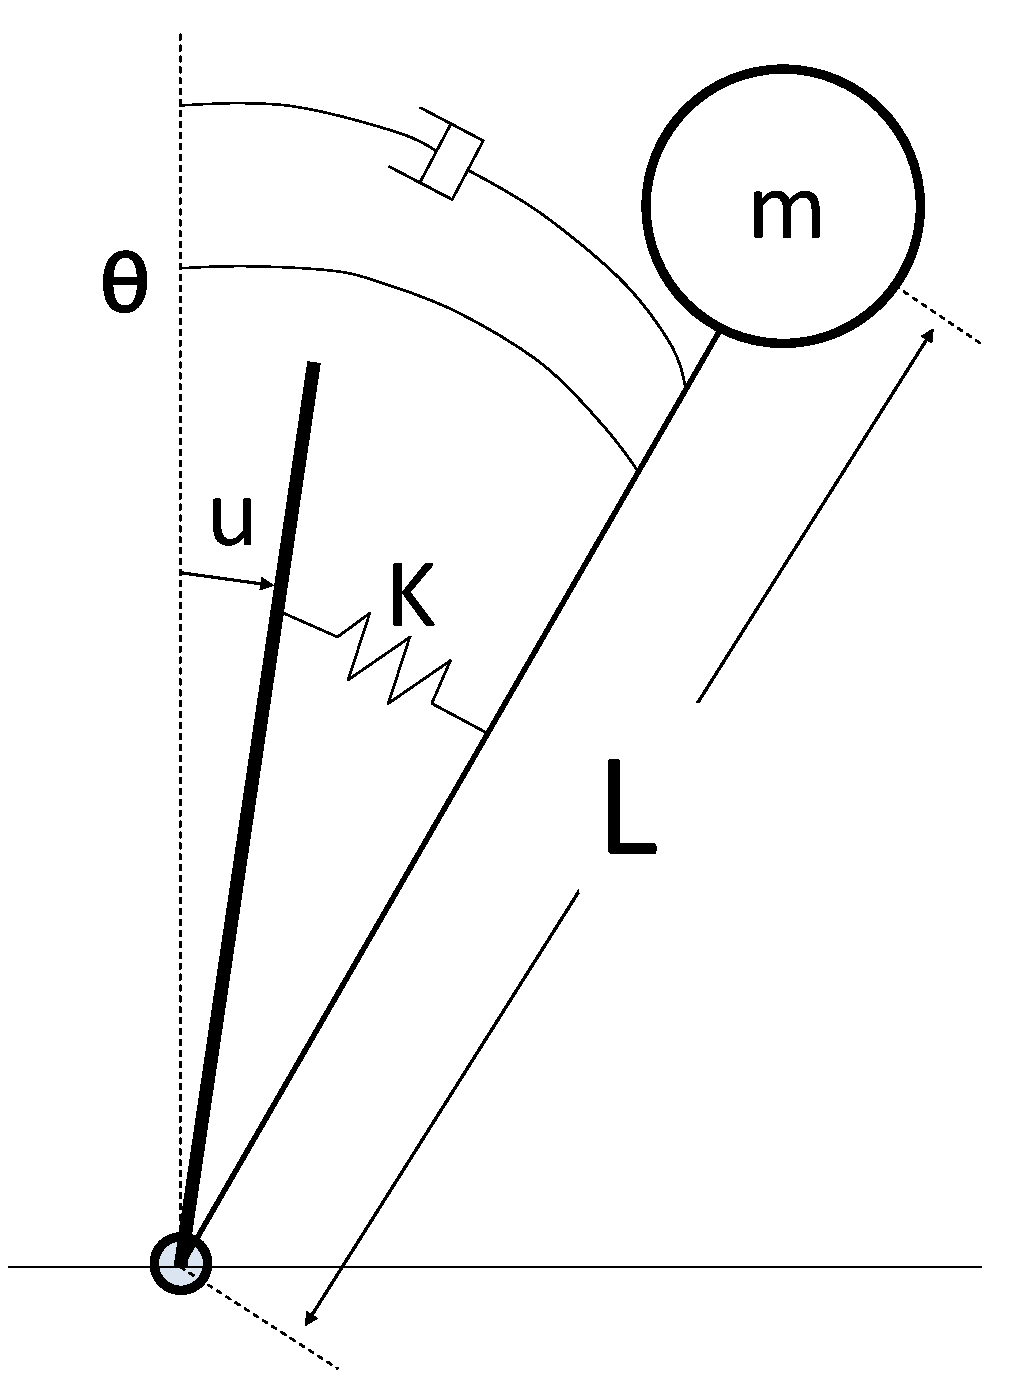
\includegraphics[width=0.5\columnwidth]{./pix/invPen3.pdf}
  \caption{Hubo modeled as a single inverted pendulum with COM located a distance $L$ from }
  \label{fig:invPen}
\end{figure}

The dynamic equation of the simplified model is assumed to be the same in both the sagittal and coronal plane.

\begin{equation}
mL^2\ddot{\theta}+C\dot{\theta}-K\theta = Ku
\end{equation}

This can be linearized and made into the transfer function:

\begin{equation}
%G(s) = \frac{\Theta(s)}{U(s)} = \frac{K}{ mL^2s^2 + Cs + (K - mgL)}
G(s) = \frac{\Theta(s)}{U(s)} = \frac{\frac{K}{mL^2}}{s^2+\frac{C}{mL^2}s + \frac{K-mgL}{mL^2}}
\end{equation}

Prior work on the model and controller for the Hubo by Cho et. al. calculated K=753 $\frac{Nm}{rad}$ and C=18 $\frac{Nm}{sec}$ using the free vibration response method\cite{5379574}.


\begin{figure}[ht]
  \centering
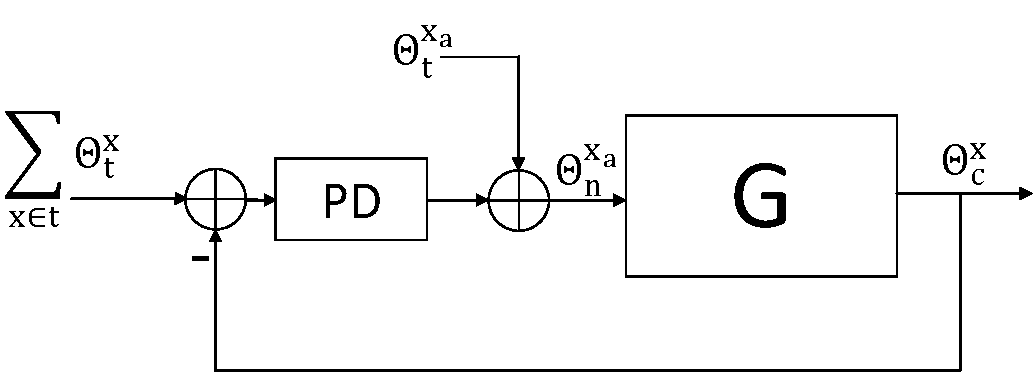
\includegraphics[width=1.0\columnwidth]{./pix/blockDiagram3.pdf}
  \caption{Block diagram of the balance controller used to balance Hubo in this work.}
  \label{fig:ctrlBlockDiagram}
\end{figure}

The control law is as follows
%ffFor the ankle roll (in the coronal plane) it is always assumed that the desired orientation of the COM is zero degrees.  Thus the roll of the IMU is taken as the error.

\begin{equation}
\theta_n^{x_a} = \theta_t^{x_a} + \left(K_p^x+sK_d^x\right)\left(\sum\limits_{x \in t} \theta_{t}^x - \theta_{c}^x\right)
%\theta_{n}^x = \theta_{t}^x + \left(K_p^x+sK_d^x\right)\left(\sum \theta_{t}^x - \theta_{c}^x\right)
%\theta_{n}^x = \theta_{t}^x + (K_p^x+sK_d^x)(\sum \theta_{t}^x - \theta_{c}^x)
%\theta_{new} = \theta_{traj} + (K_p+sK_d)(\sum \theta_{leg} - \theta_{IMU})
\end{equation}

Where $\theta_t$ is the desired trajectory of the lower body (pitch or roll), $x$ denotes pitch or roll and $x_a$ denotes pitch or roll on the ankle.  $\theta_{c}$ is the orientation of the center of mass in the global frame.  $\theta_n$ is the resulting trajectory.  $K_p$ and $K_d$ are the proportional and derivative gains.  The resulting control allows for a stable stance even with perturbations from upper body motions.

\subsection{Human to Humanoid Kinematic Mapping}\label{sec:sec:mocap}

Motion capture (MoCap) systems can be used to generate human-like motions and map those motion to humanoids\cite{1545060,Polland2002}.  
Fig.~\ref{fig:mocap-joints} shows the Hubo's kinematic structure (left) and the human (MoCap) kinematic structure(left).
The human has 3-DOF at each joint while the humanoid has limited DOF at each corresponding joint.
Some of the challenges in mapping between the human kinematic structure (from MoCap) to a humanoid's kinematic structure are:

\begin{itemize}
	\item The difference in the total degree of freedom (DOF). 
	\item	The difference in the kinematics descriptions. 
	\item	The different Kinematic constraints.
\end{itemize}

%Gaertner et. al.\cite{5756898} uses an intermediate model (Master Motor Map) to decouple motion capture data for further post-processing tasks. 
Our approach is to: 
a) Chose a set MoCap model.  
b) Preform motions where the pitch motions are decoupled (roll and yaw stays constant), avoids singularities and robot joint position limitations.  
c) Combine joint values for near by joints (reduce the model to the same DOF as the robot).  
d) Some tests require the addition of static offsets to joints to ensure the zero-moment-point (ZMP) criteria is satisfied as stated in Section~\ref{sec:sec:balance}

\begin{figure}[t]
  \centering
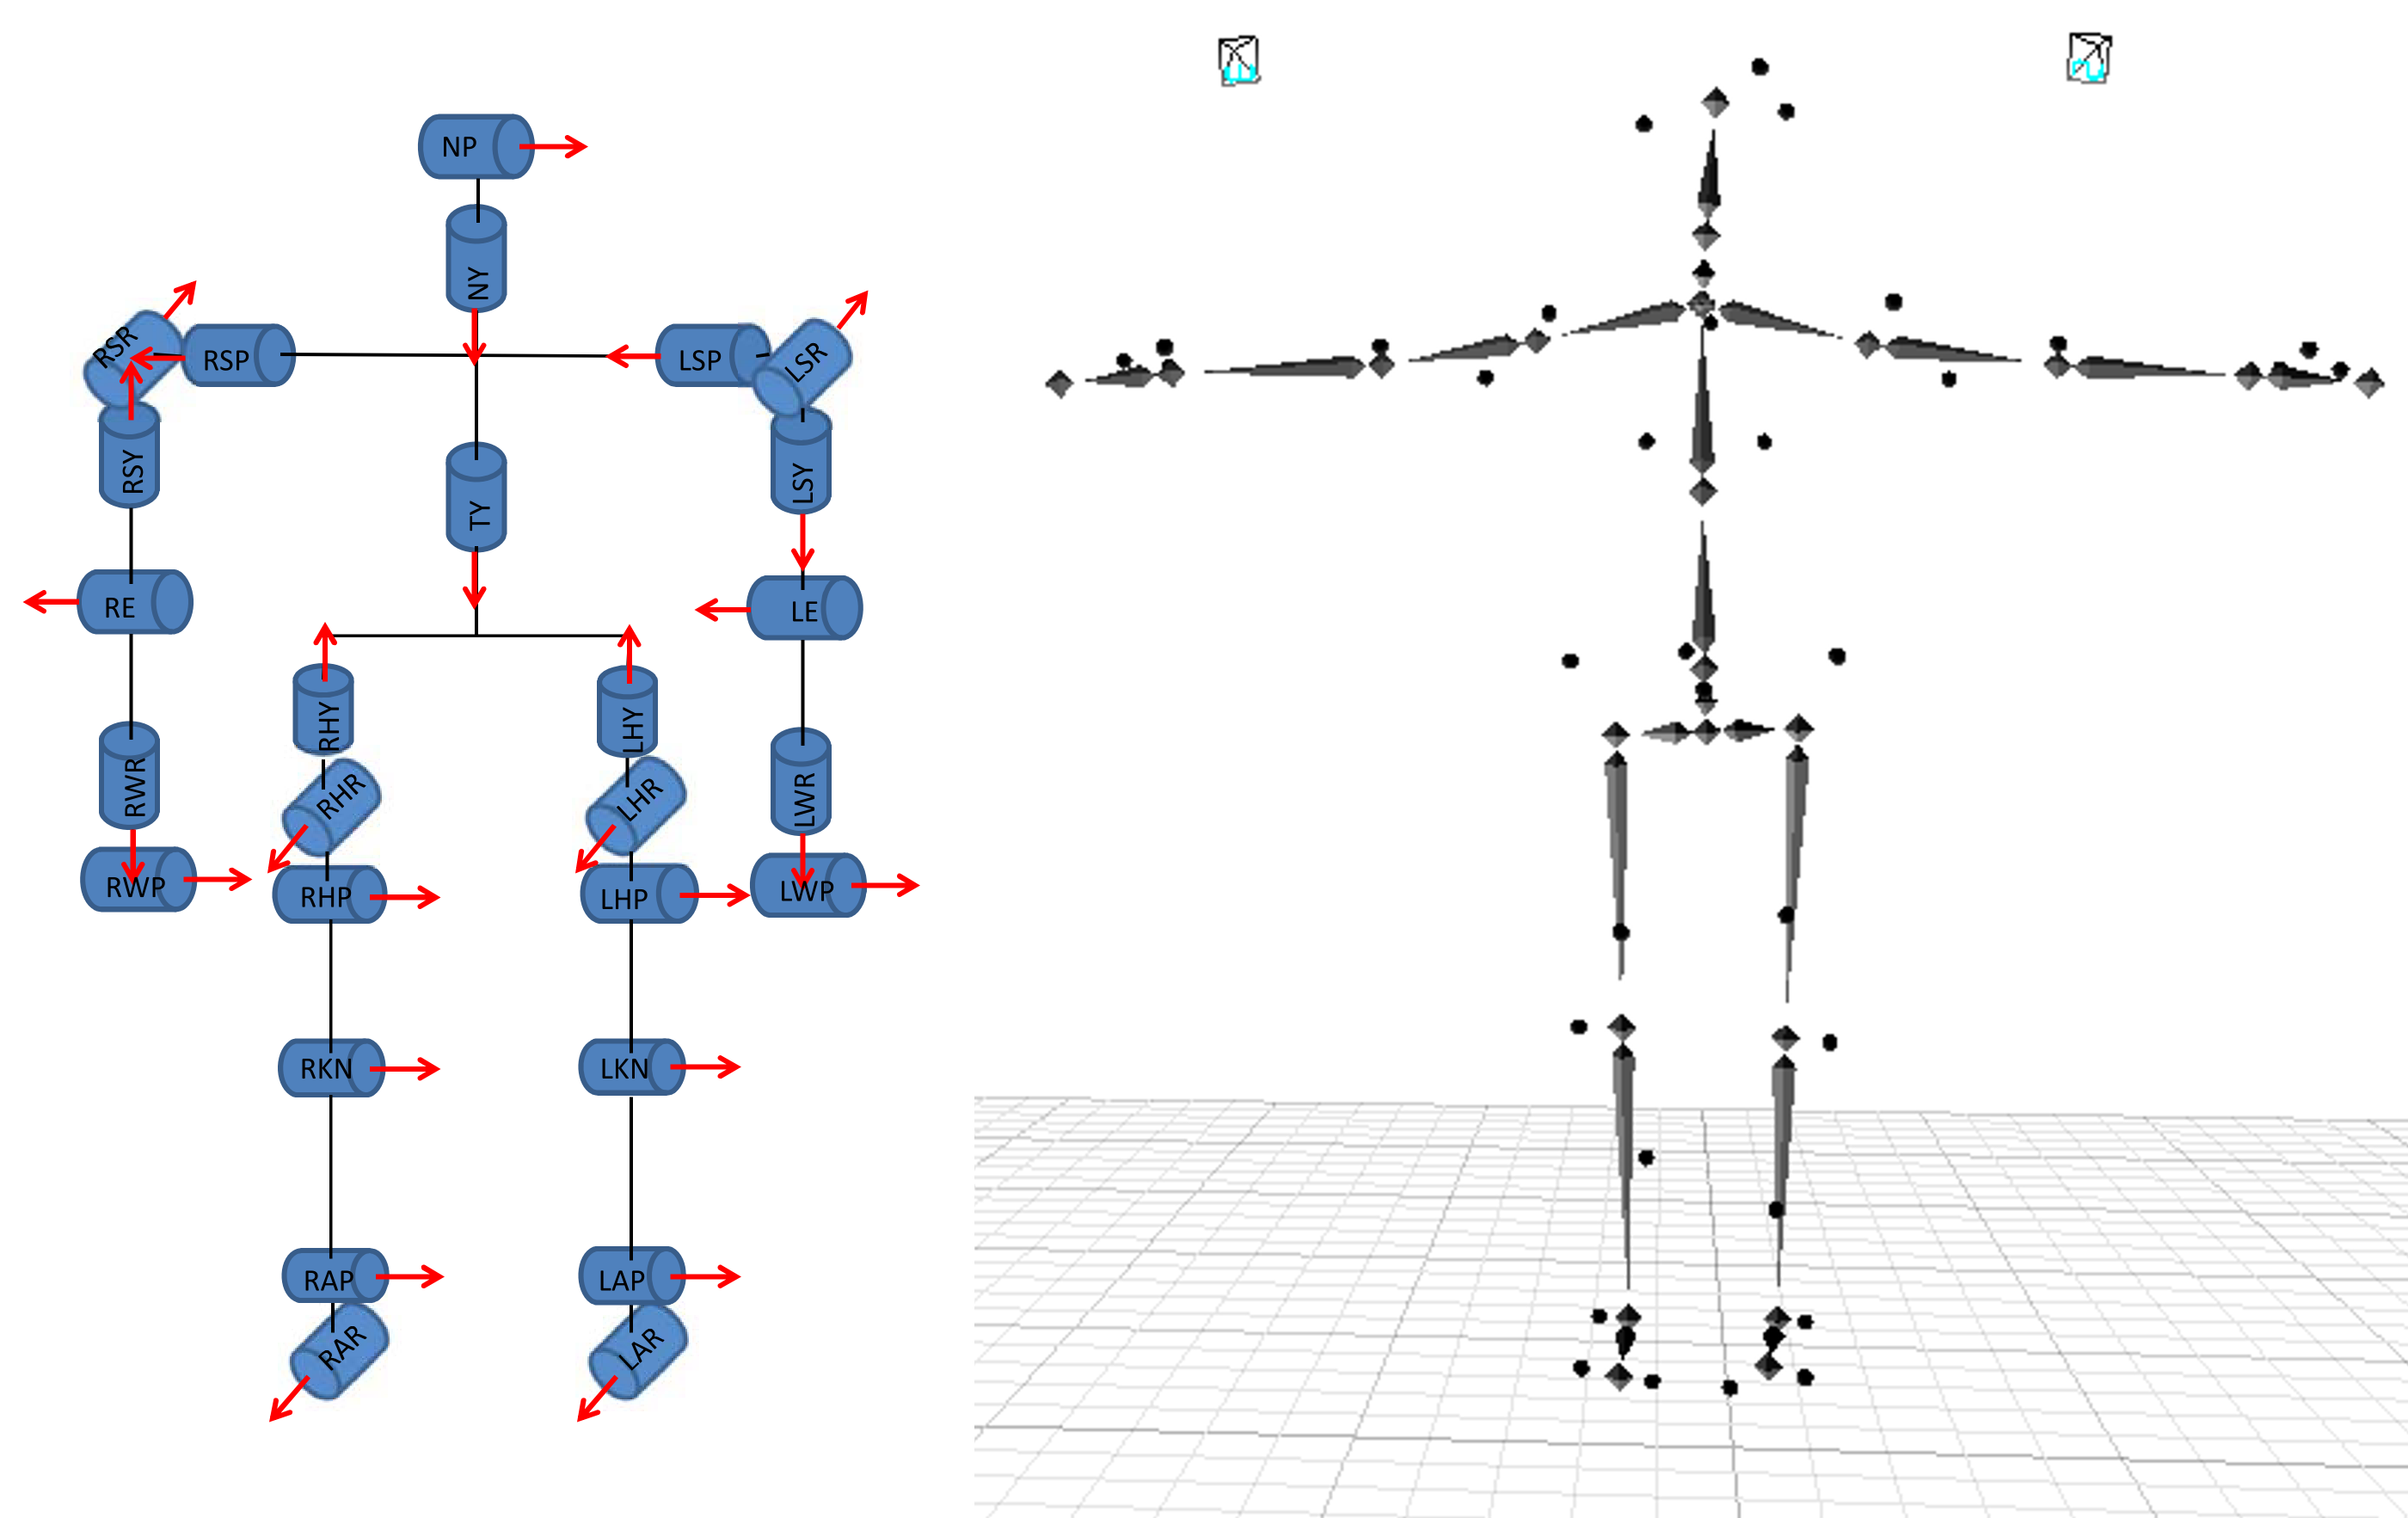
\includegraphics[width=1.0\columnwidth]{./pix/mocapJoints.png}  \caption{Left: Jaemi Hubo joint order and orientation using right hand rule.  Right: Motion capture model of human figure}
  \label{fig:mocap-joints}
\end{figure}



To test this method we used a human subject to throw a ball using upper and lower body movements.  
All motions were in the sagittal plane to keep pitch joints decoupled.  
To avoid the robot's joint limit of $\pm180^o$ an underhand throwing motion was used.
Fig.~\ref{fig:mocap-underhand} shows the human throwing the ball and the robot throwing the ball to the mapped motion of the human.

\begin{figure}[t]
  \centering
\includegraphics[width=1.0\columnwidth]{./pix/mocap/throwmocap3.png}
%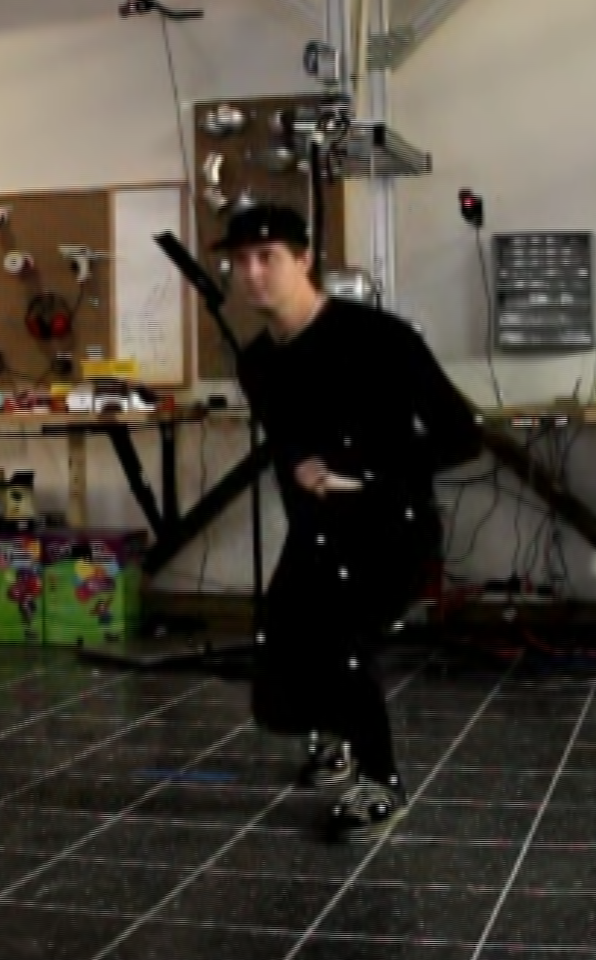
\includegraphics[width=0.33\columnwidth]{./pix/mocap/1a.png}
%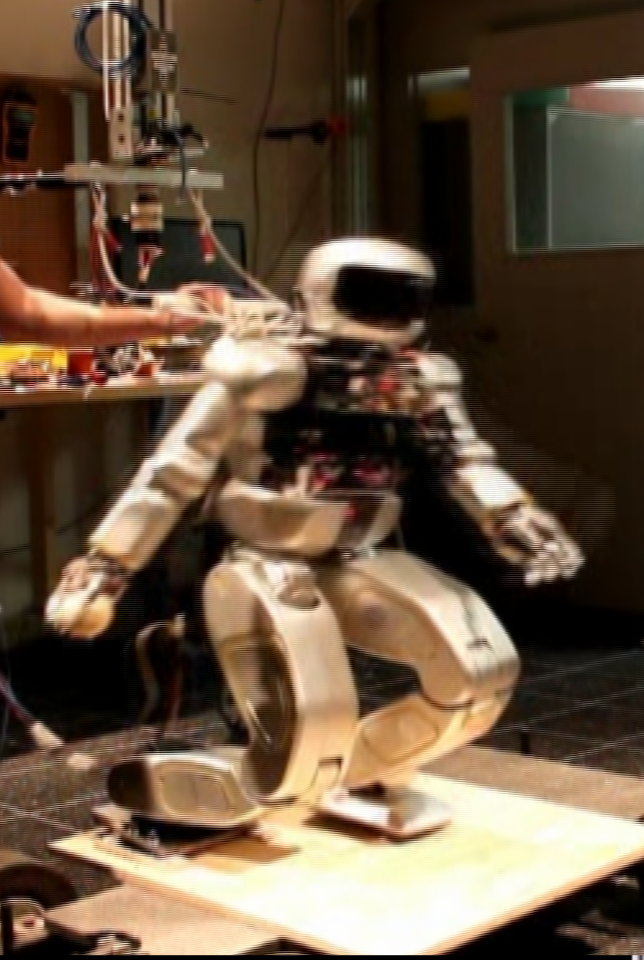
\includegraphics[width=0.33\columnwidth]{./pix/mocap/1b.png}
%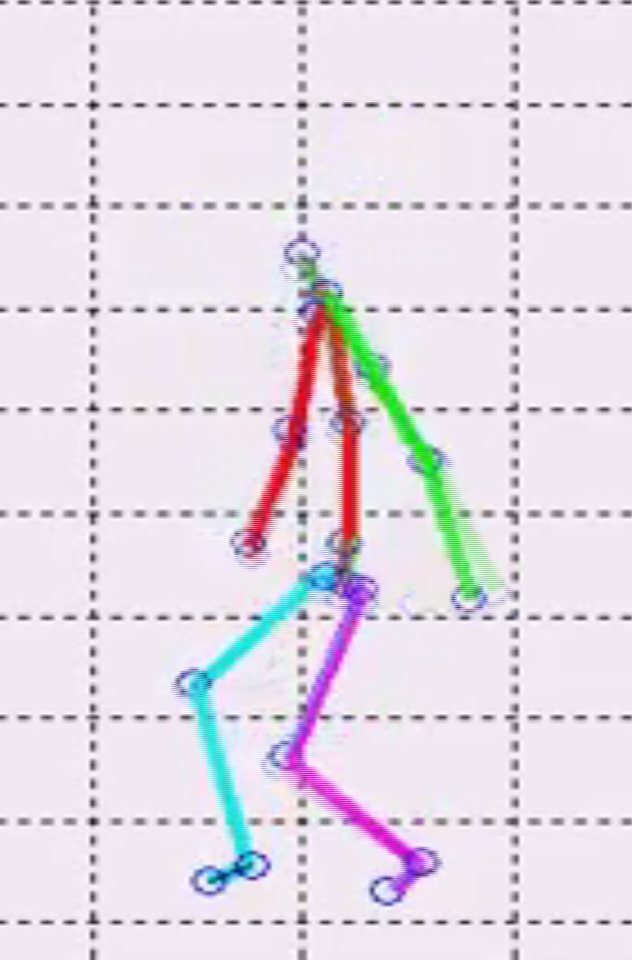
\includegraphics[width=0.33\columnwidth]{./pix/mocap/1c.png} 
%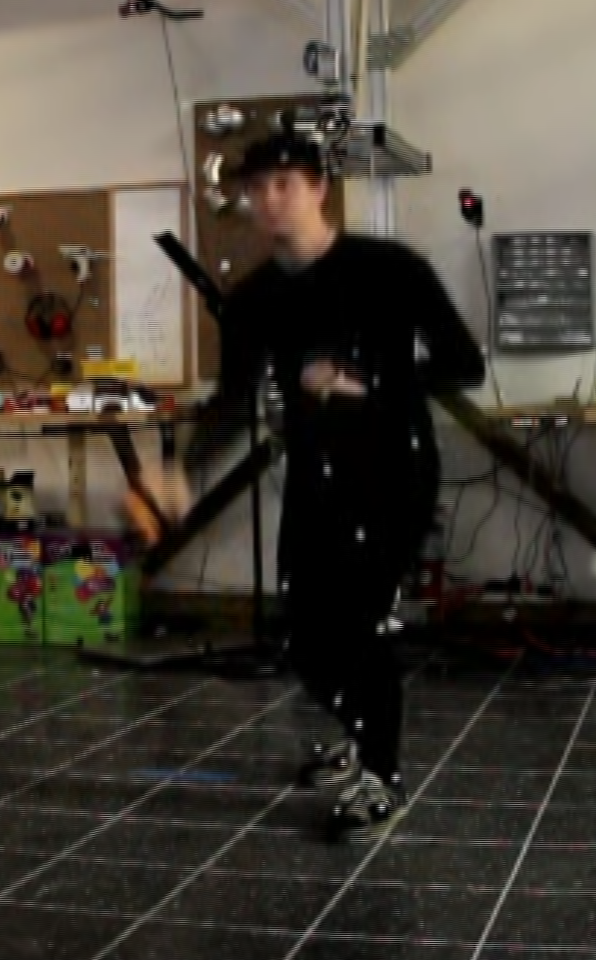
\includegraphics[width=0.33\columnwidth]{./pix/mocap/2a.png}
%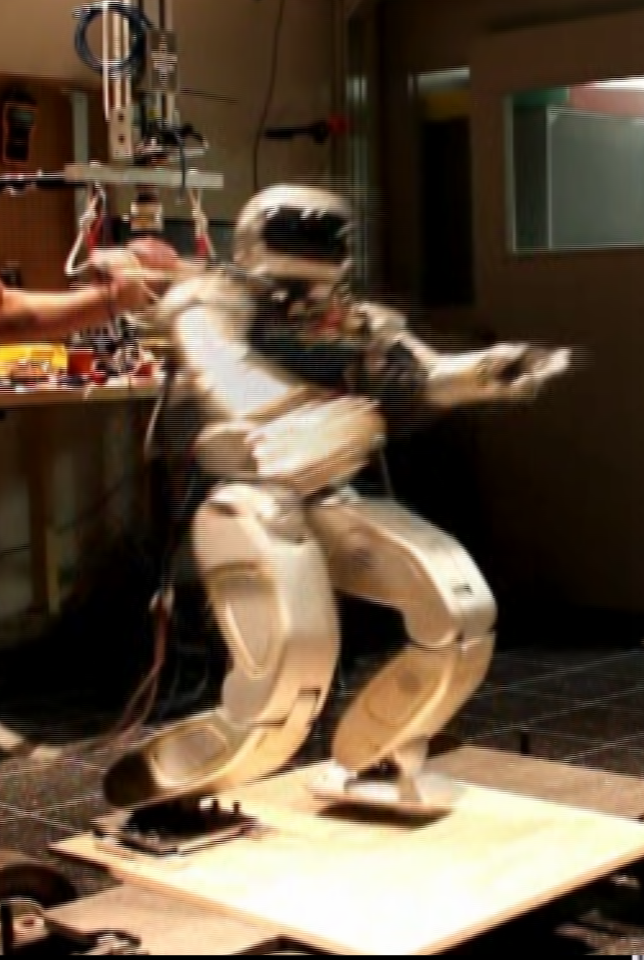
\includegraphics[width=0.33\columnwidth]{./pix/mocap/2b.png}
%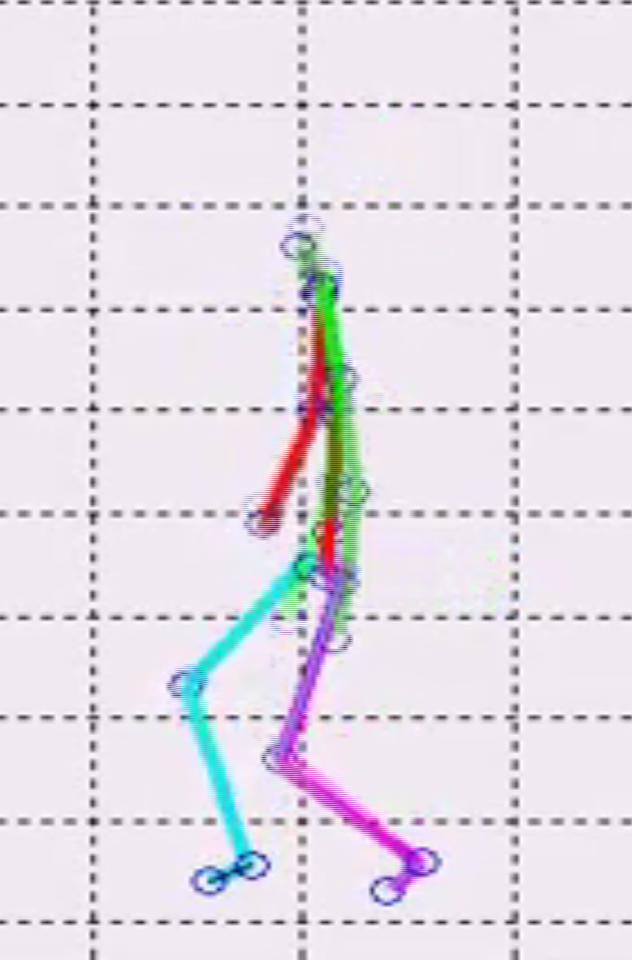
\includegraphics[width=0.33\columnwidth]{./pix/mocap/2c.png} 
%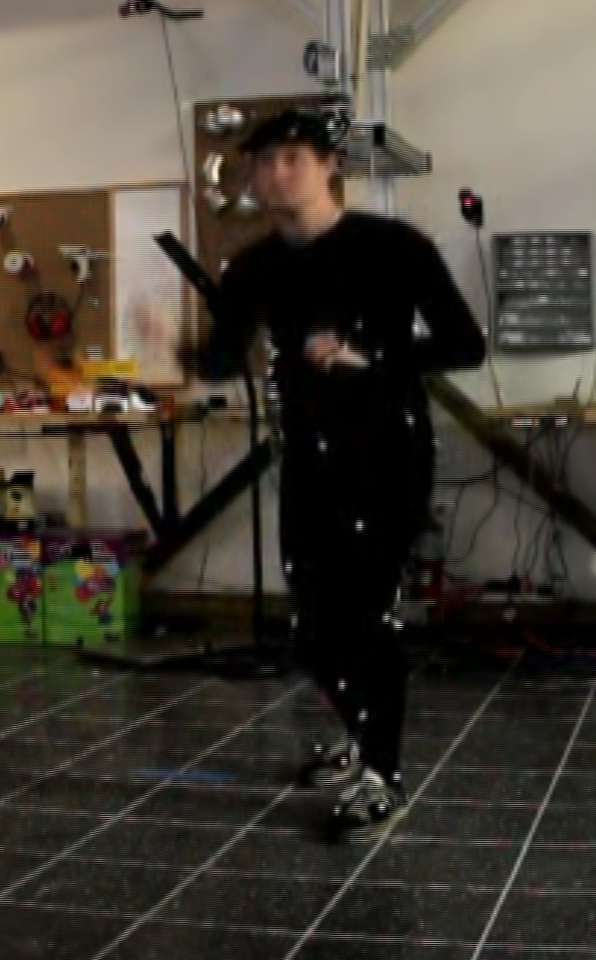
\includegraphics[width=0.33\columnwidth]{./pix/mocap/3a.png}
%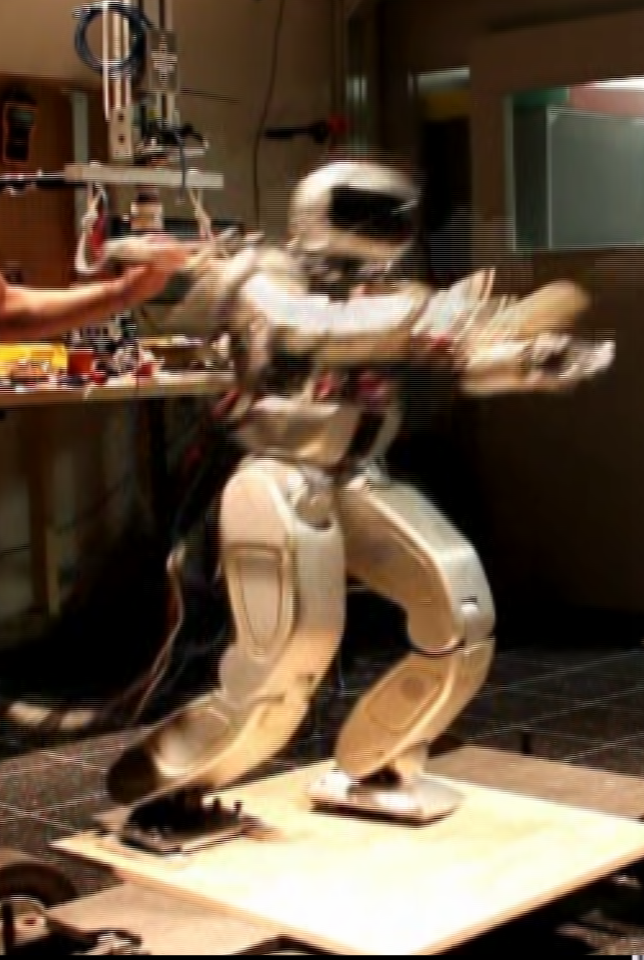
\includegraphics[width=0.33\columnwidth]{./pix/mocap/3b.png}
%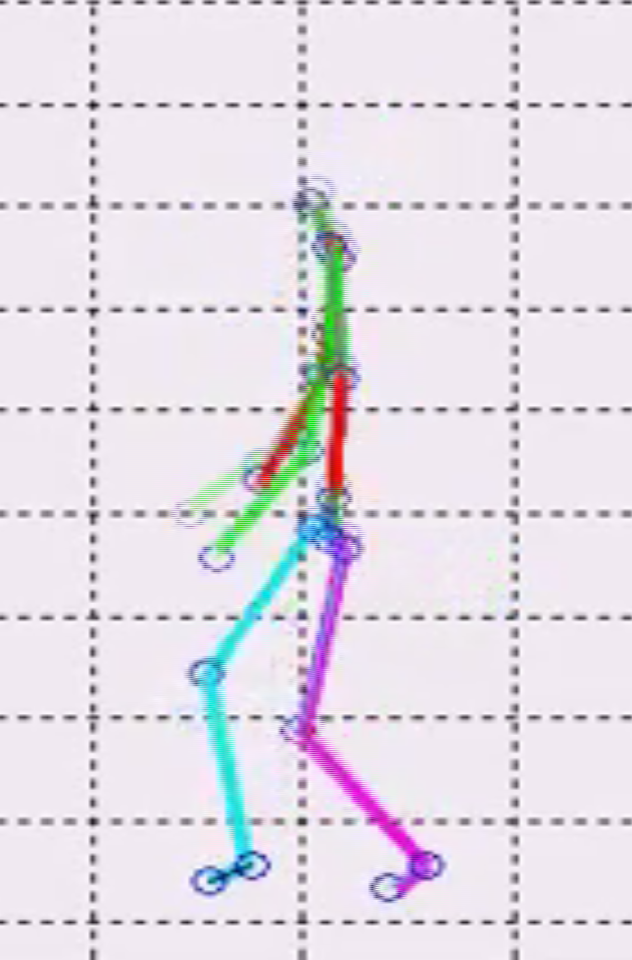
\includegraphics[width=0.33\columnwidth]{./pix/mocap/3c.png} 
%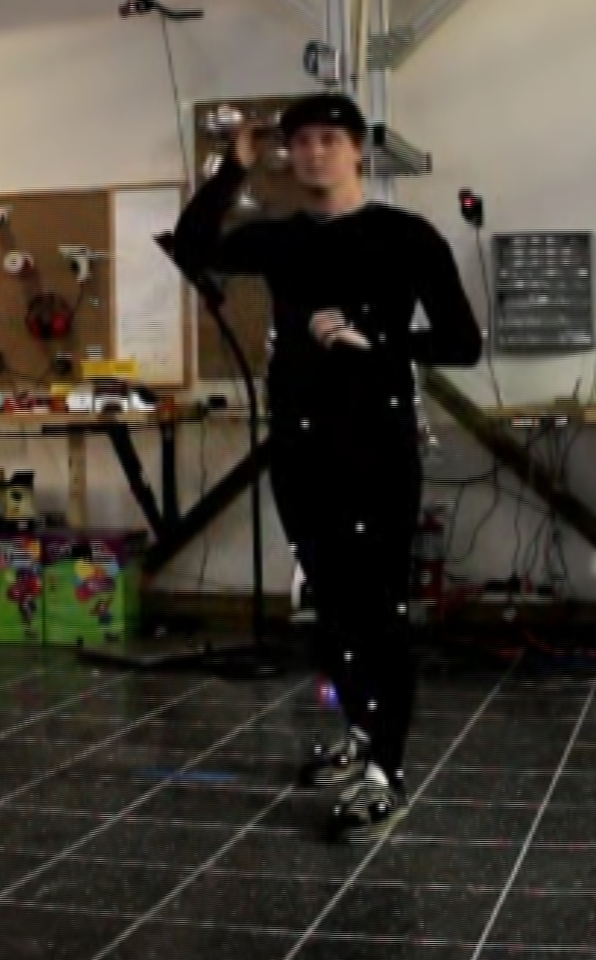
\includegraphics[width=0.33\columnwidth]{./pix/mocap/4a.png}
%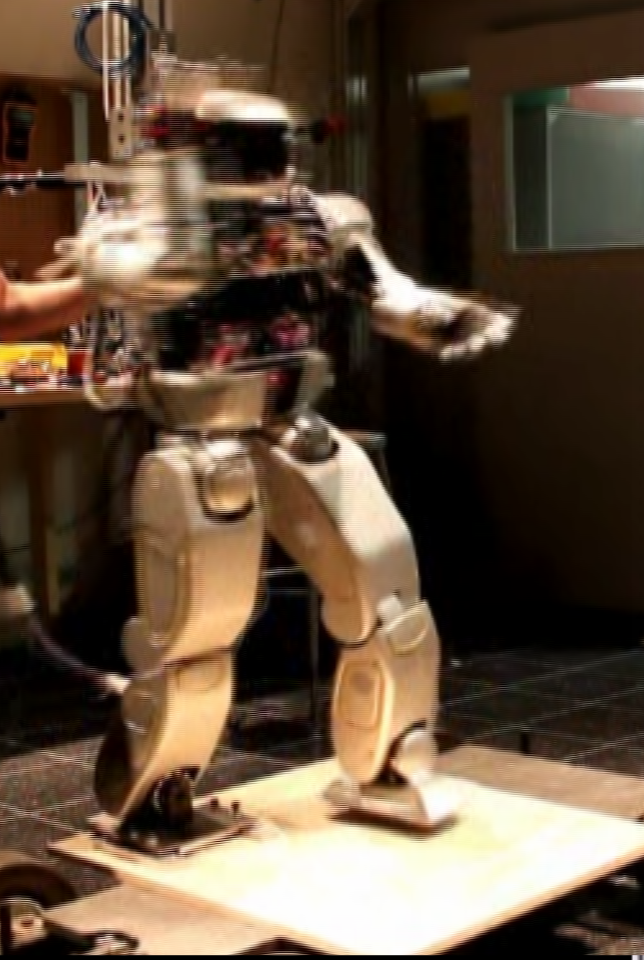
\includegraphics[width=0.33\columnwidth]{./pix/mocap/4b.png}
%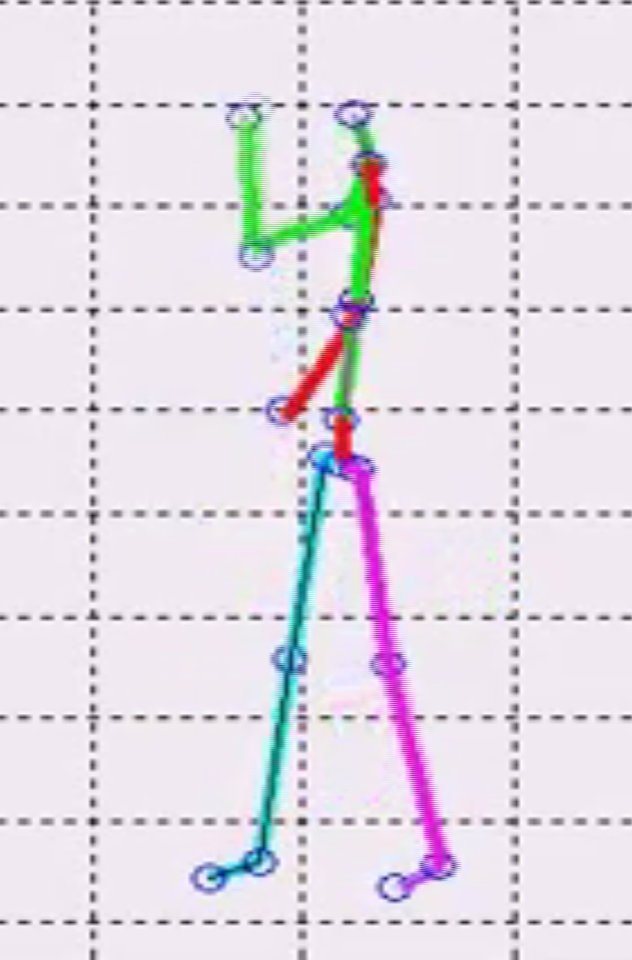
\includegraphics[width=0.33\columnwidth]{./pix/mocap/4c.png} 
  \caption{(Left to Right): (1) Human throwing underhand in sagittal plane while being recorded via a motion capture system.  (2) Recorded trajectory mapped to high degree of freedom model.  (3) High degree of freedom model mapped to lower degree of freedom OpenHUBO.  (4) Resulting trajectory and balancing algorithm run on Hubo.}
  \label{fig:mocap-underhand}
\end{figure}

To ensure balance throughout the motion the balance controller as described in Section~\ref{sec:sec:balance} was applied and the static ZMP criteria was checked for the entire trajectory.
The human subject threw the ball approximately eight feet (244 cm).  
The mapping of the latter motion caused the robot to throw the ball approximately five feet (152 cm).
The discrepancy comes from the proportional difference in limb length from the human to the robot.
%A side by side video of the human and the robot throwing the ball is available for viewing on the this papers's homepage\footnote{MoCap to Robot (Video): http://danlofaro.com/urai2012/\#mocap}.





\subsection{\bf Throwing Using Sparse Reachable Map}\label{sec:sec:srm}

A Sparse Reachable Map (SRM) is used to create a collision free trajectories while having the end-effector reach a desired velocity as discribed in Lofaro et. al.\cite{dlofaro-srm}.
The SRM has been shown to be a viable method for trajectory generation for high degree of freedom, high-gain position controlled robots.  This remains true when operating without full knowledge of the reachable area as long as a good collision model of the robot is available. 
The end-effector velocity (magnitude and direction) is specified as well as a duration of this velocity. 
The SRM is created by making a sparse map of the reachable end-effector positions in free space and the corresponding poses in joint space by using random sampling in joint space and forward kinematics. 
The desired trajectory in free space is placed within the sparse map with the first point of the trajectory being a known pose from the original sparse map. 

\begin{equation}
L_d(0) \in SRM
\end{equation}

$L_d(0)$ is known both in joint space and in free space.
The Jacobian Transpose Controller method of inverse kinematics as described by Wolovich et al.\cite{4048118} is then used to find the subsequent joint space values for the free space points in the trajectory. 

\begin{equation}
q_1 = q_0 + \dot{q}_0 = q_0 + kJ^Te|_{x_0}^{x_1}
\end{equation}

Where $q_0$ and $x_0$ is the current pose and corresponding end-effector position respectively.  $q_1$ is the next pose for the next desired end-effector position $x_1$.
Each desired end-effector position $x$ must be within a euclidean distance $d$ (user defined) from any point in the SRM.

\begin{equation}
min \left(|x - SRM| \right) < d
\end{equation}

If one of the points in $x$ fails this criteria a new random point is chosen for $L_d(0)$ and the process is repeated.

Each pose in the trajectory is checked against the collision model to guarantee no self-collisions.  The collision model is based on the OpenRAVE model of the Hubo platform called OpenHUBO, see Fig~\ref{fig:vHubo}.

\begin{figure}[ht]
  \centering
%\includegraphics[width=0.5\columnwidth]{./pictures/hubo1s.png}\includegraphics[width=0.5\columnwidth]{./pictures/hubo2s.png}


%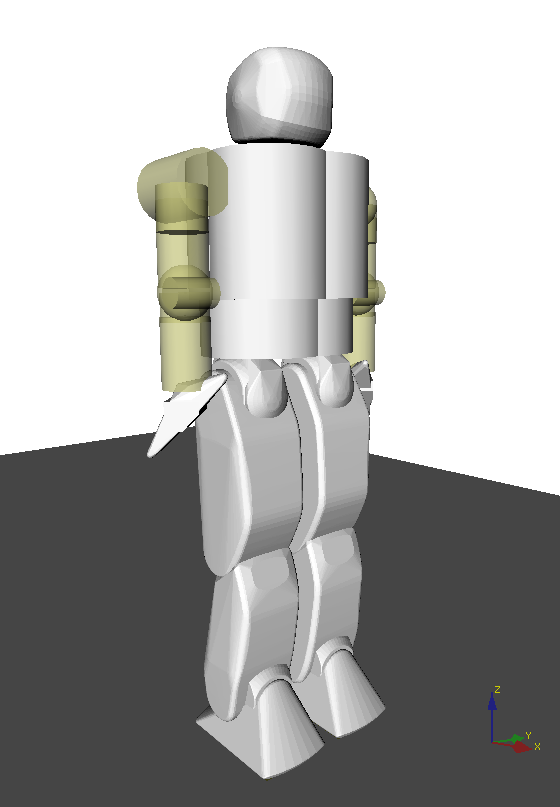
\includegraphics[width=0.5\columnwidth]{./pix/hCol.png}%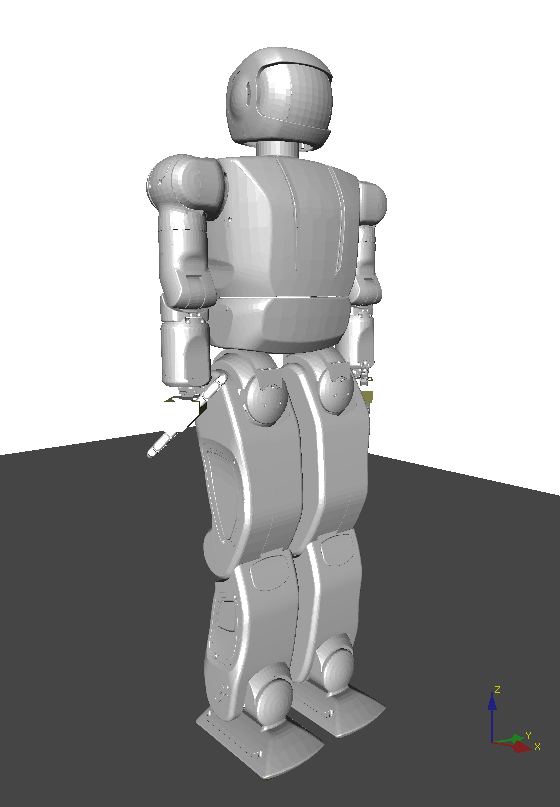
\includegraphics[width=0.5\columnwidth]{./pix/hBody.png}

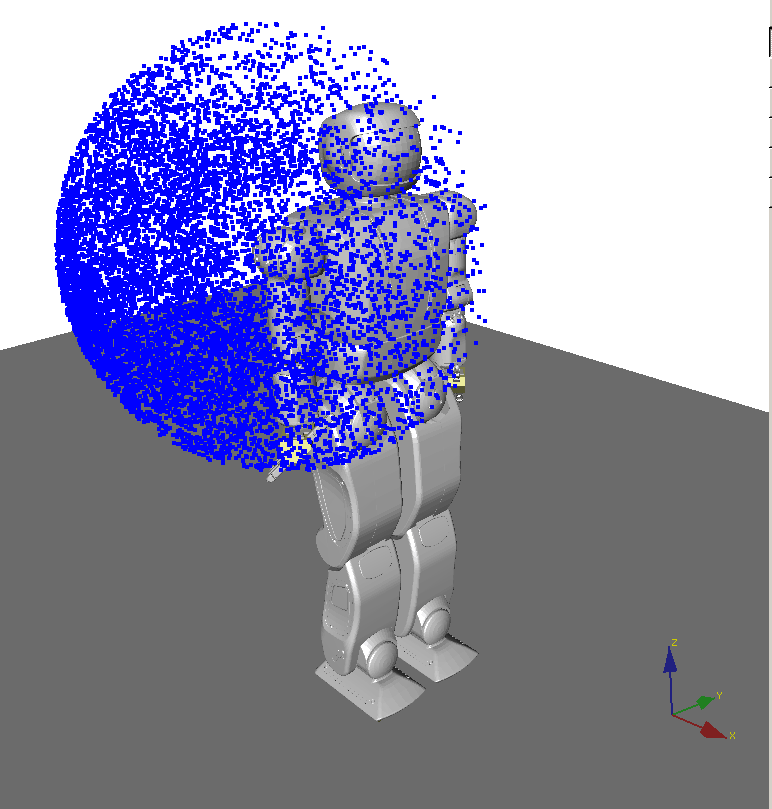
\includegraphics[width=0.36\columnwidth]{./pix/SRM.png}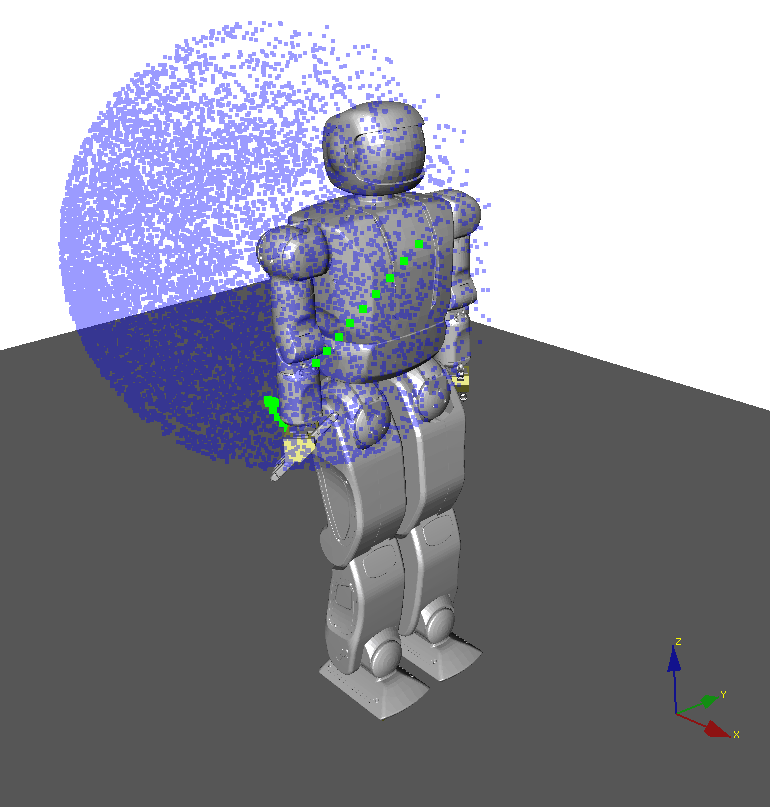
\includegraphics[width=0.36\columnwidth]{./pix/ThrowTrajDiag.png}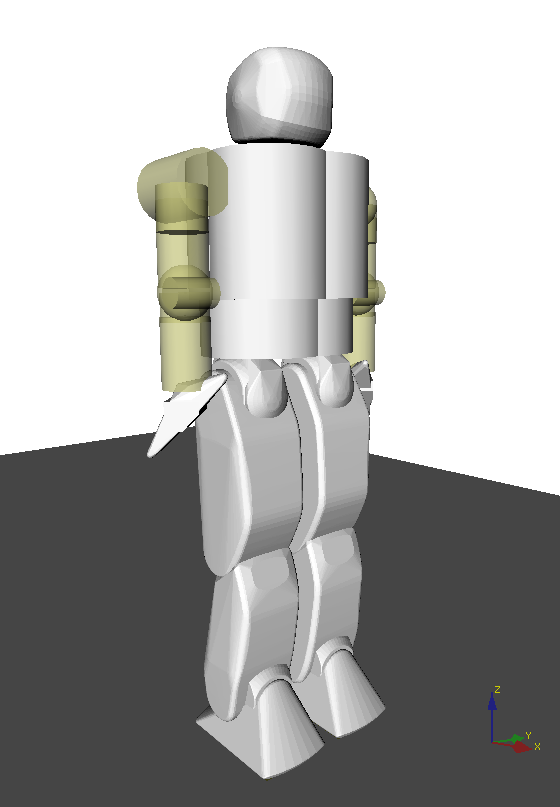
\includegraphics[width=0.28\columnwidth]{./pix/hCol.png}
  \caption{OpenRAVE model of Hubo KHR-4. Left: Model with SRM of right arm.  Center: SRM (blue) with setup and velocity phase trajectories (green) Right: Collision Geometry\cite{dlofaro-srm}  }
  
  %\caption{OpenHUBO - OpenRAVE model of Hubo KHR-4.  Left: Collision Geometry.  Right: Model with protective shells\cite{dlofaro-srm}.  }
  \label{fig:vHubo}
\end{figure}

The commanded trajectory produces the desired velocity of 4.9 m/s at 60$^o$.  This was then tested on the OpenHUBO and on the Jaemi Hubo platform, Fig~\ref{fig:3dThrowReal} and Fig~\ref{fig:3dThrowReal} respectively.



%\begin{figure}[ht]
%  \centering
%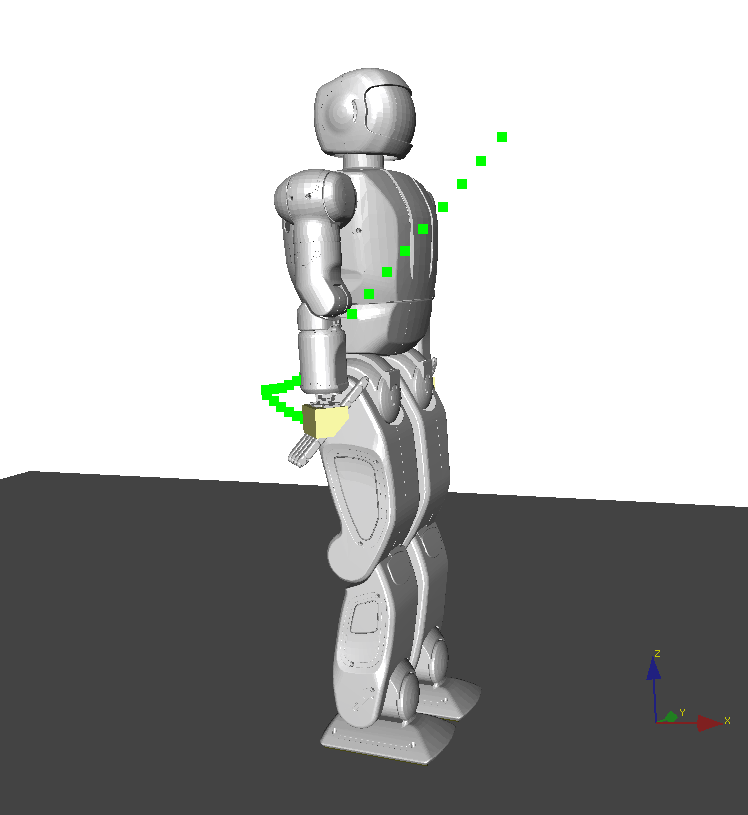
\includegraphics[width=0.25\columnwidth]{./pix/ddFinal/vHside1.png}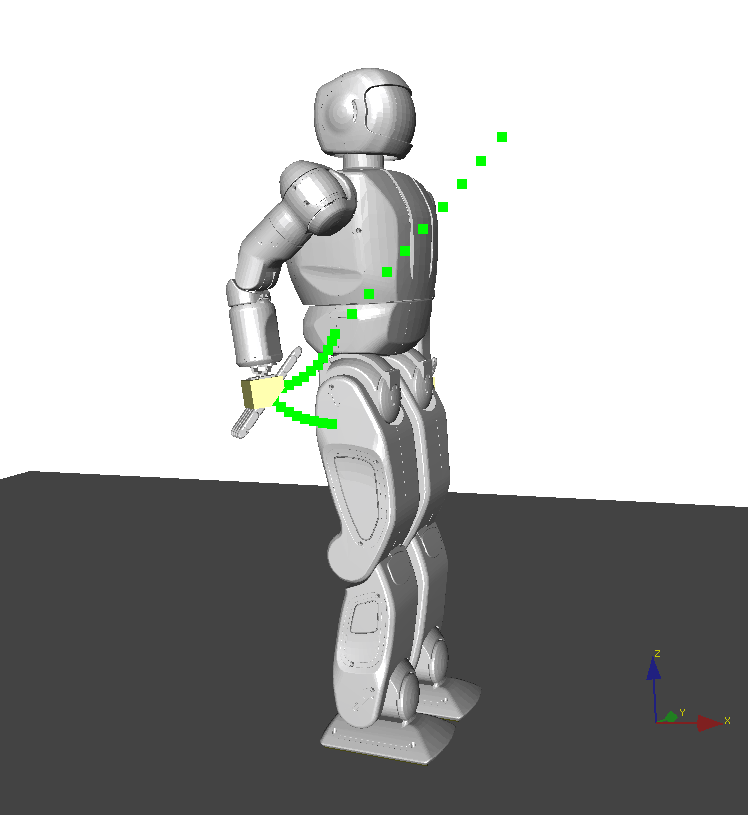
\includegraphics[width=0.25\columnwidth]{./pix/ddFinal/vHside3.png}%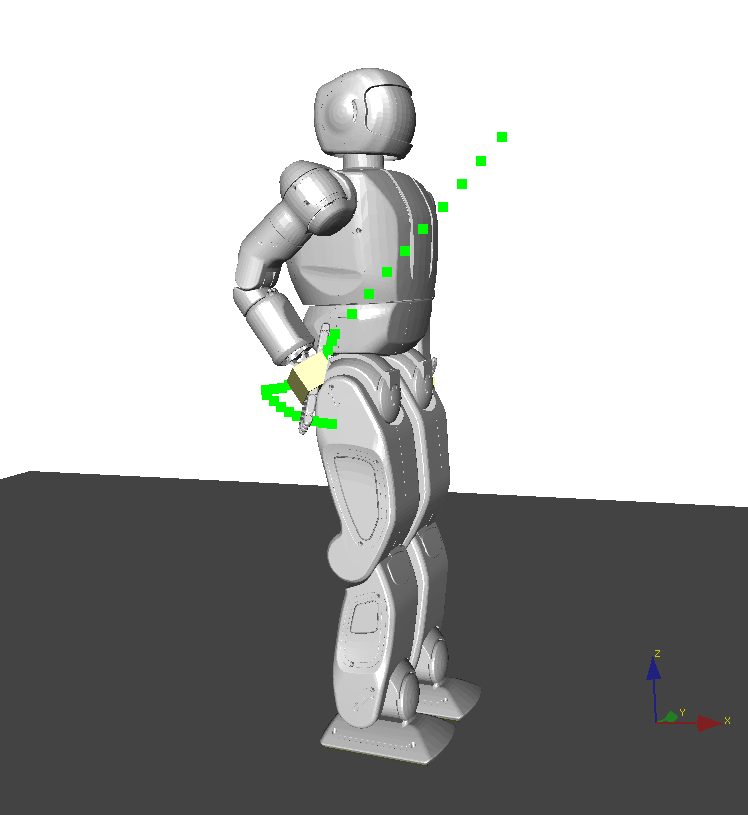
\includegraphics[width=0.25\columnwidth]{./pix/ddFinal/vHside4.png}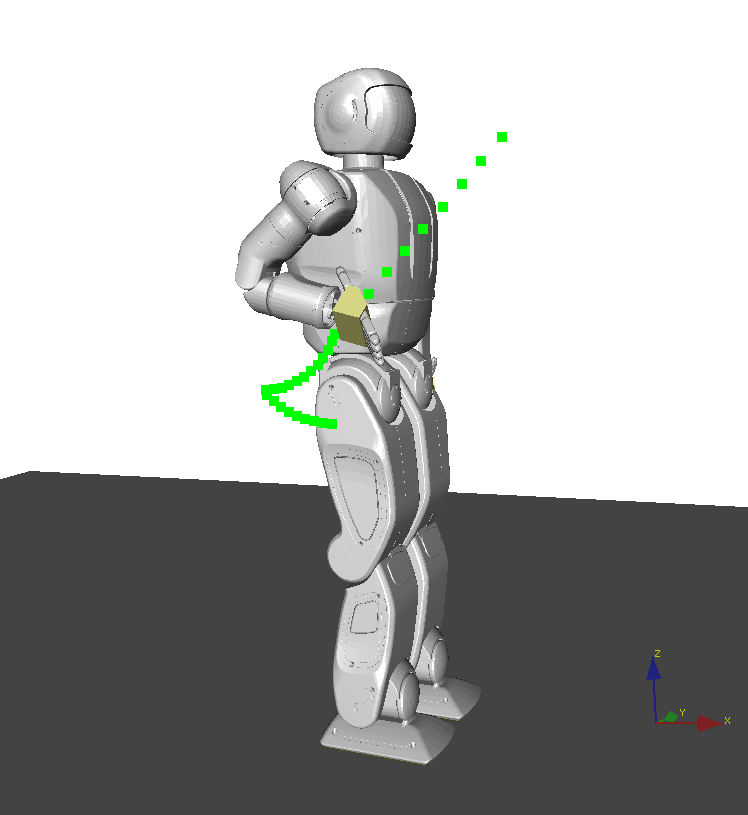
\includegraphics[width=0.25\columnwidth]{./pix/ddFinal/vHside5.png}
%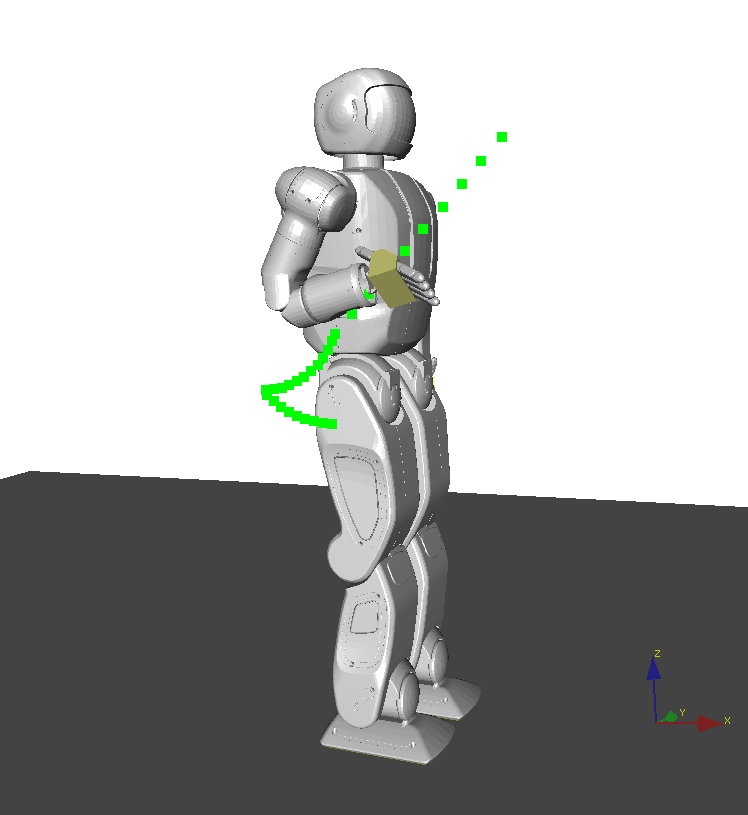
\includegraphics[width=0.25\columnwidth]{./pix/ddFinal/vHside6.png}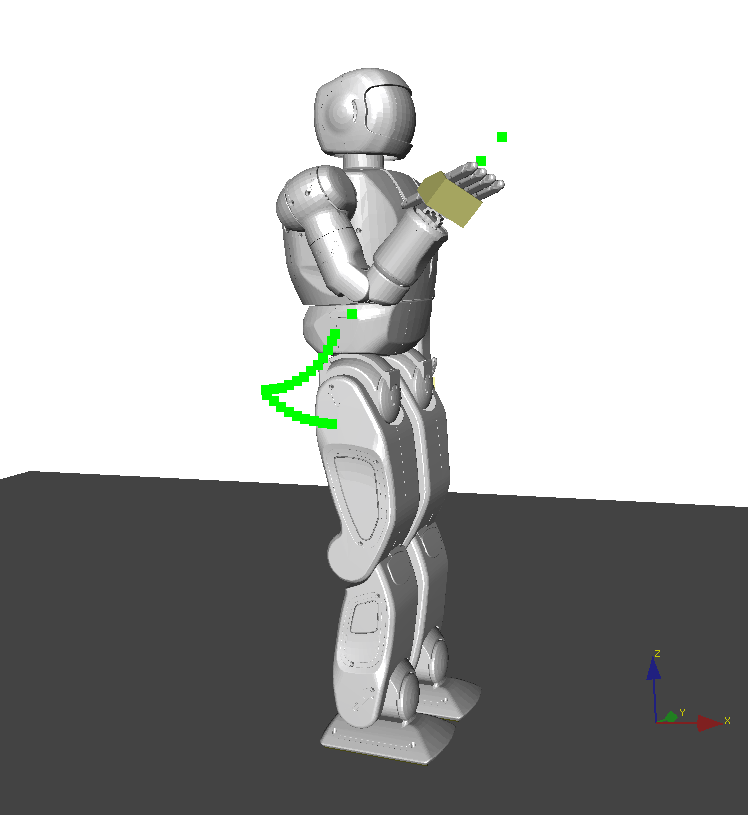
\includegraphics[width=0.25\columnwidth]{./pix/ddFinal/vHside7.png}%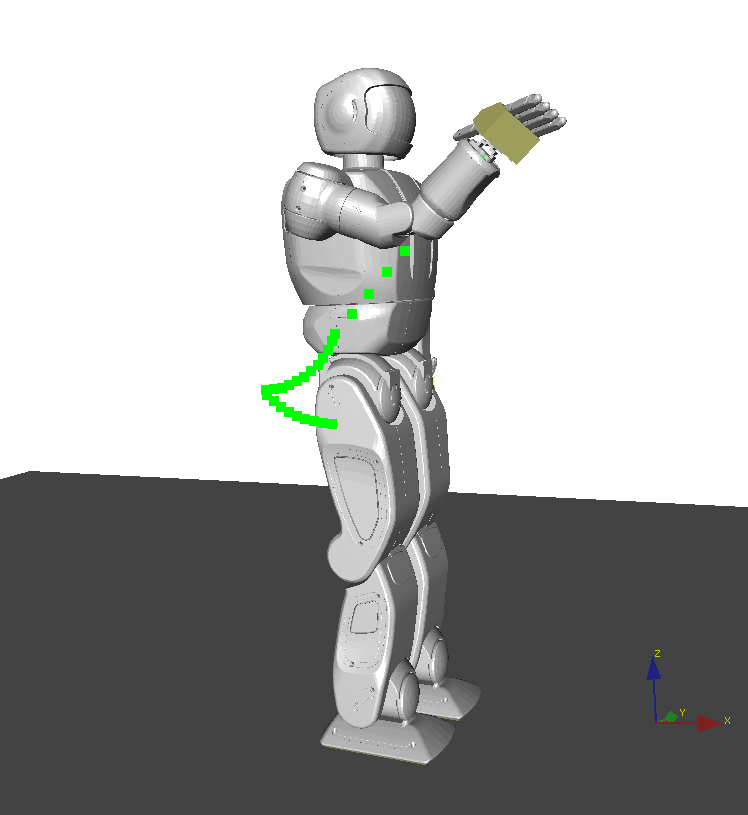
\includegraphics[width=0.25\columnwidth]{./pix/ddFinal/vHside9.png}
%  \caption{OpenHUBO running the throwing trajectory immediately after the setup phase is completed.  $x_0$ is top left.  Frames are read left to right and have a $\Delta t$ of %0.15s\cite{dlofaro-srm}}
%  \label{fig:fThrow}
%\end{figure}

\begin{figure}[ht]
  \centering
%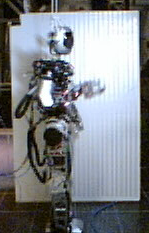
\includegraphics[width=0.25\columnwidth]{./pix/slowMotion/1.png}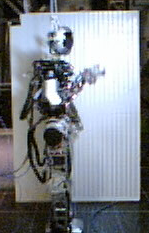
\includegraphics[width=0.25\columnwidth]{./pix/slowMotion/2.png}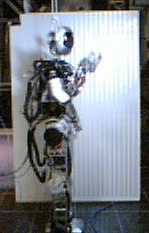
\includegraphics[width=0.25\columnwidth]{./pix/slowMotion/3.png}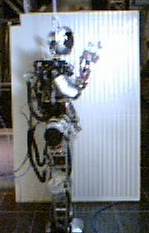
\includegraphics[width=0.25\columnwidth]{./pix/slowMotion/4.png}
%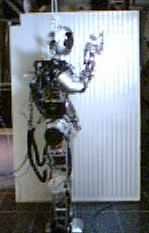
\includegraphics[width=0.25\columnwidth]{./pix/slowMotion/5.png}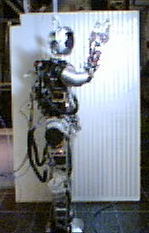
\includegraphics[width=0.25\columnwidth]{./pix/slowMotion/6.png}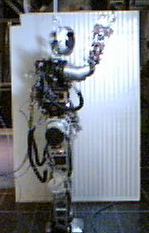
\includegraphics[width=0.25\columnwidth]{./pix/slowMotion/7.png}

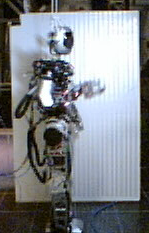
\includegraphics[width=0.25\columnwidth]{./pix/slowMotion/1.png}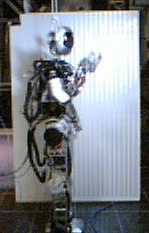
\includegraphics[width=0.25\columnwidth]{./pix/slowMotion/3.png}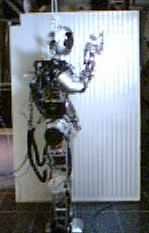
\includegraphics[width=0.25\columnwidth]{./pix/slowMotion/5.png}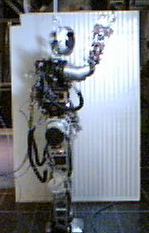
\includegraphics[width=0.25\columnwidth]{./pix/slowMotion/7.png}
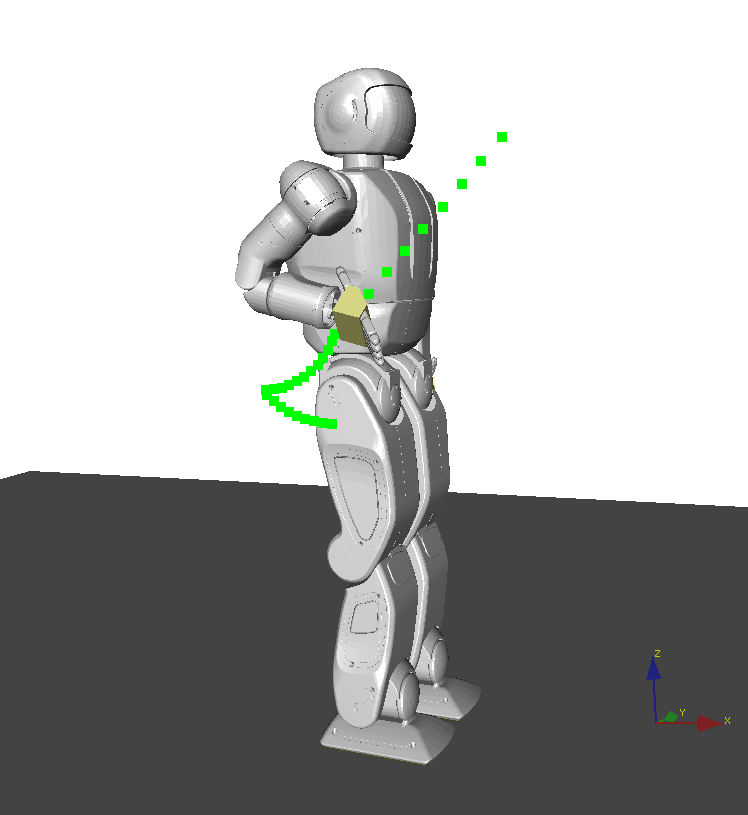
\includegraphics[width=0.25\columnwidth]{./pix/ddFinal/vHside5.png}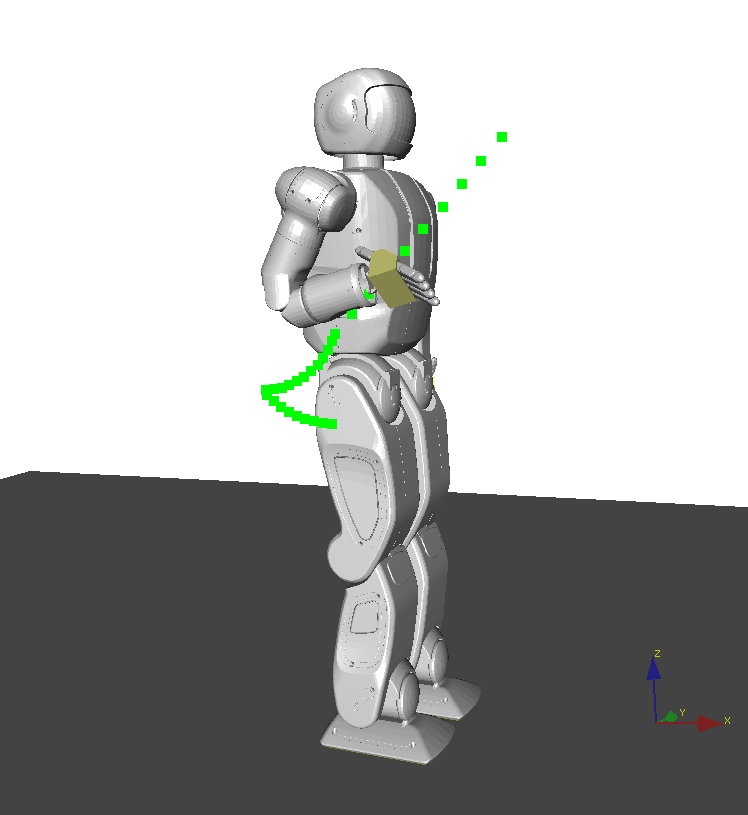
\includegraphics[width=0.25\columnwidth]{./pix/ddFinal/vHside6.png}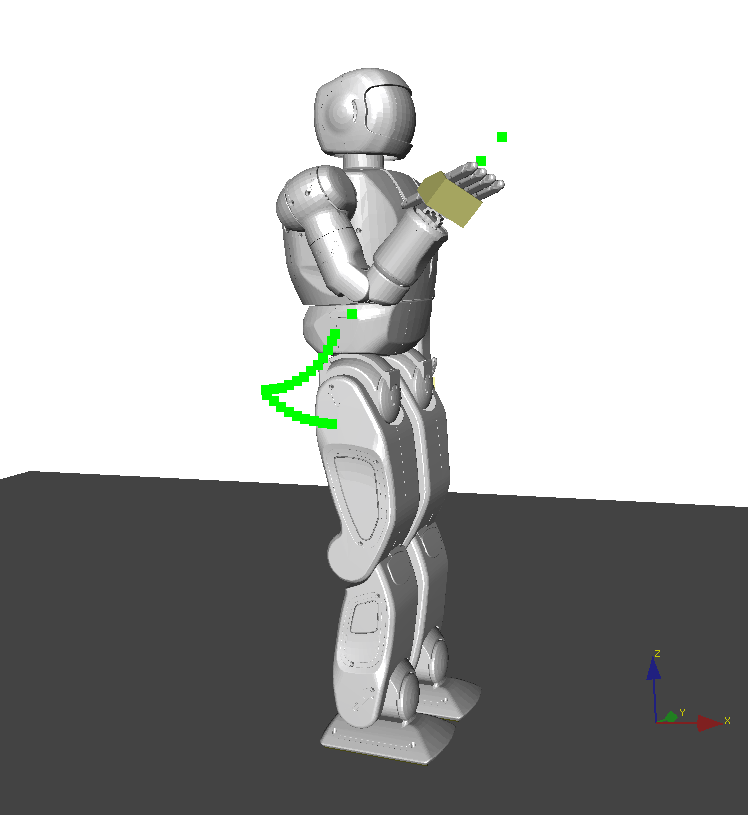
\includegraphics[width=0.25\columnwidth]{./pix/ddFinal/vHside7.png}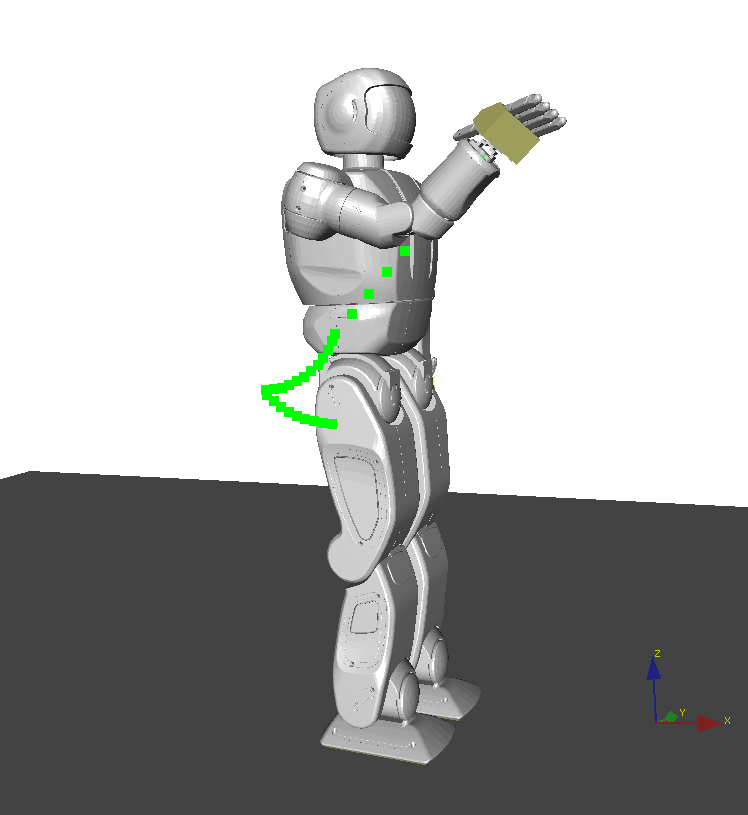
\includegraphics[width=0.25\columnwidth]{./pix/ddFinal/vHside9.png}

  \caption{(Top Row) Jaemi Hubo and (Bottom Row) OpenHUBO running the throwing trajectory immediately after the setup phase is completed.  $x_0$ is top left.  Frames are read left to right and have a $\Delta t$ of 0.15 sec\cite{dlofaro-srm}}
  \label{fig:3dThrowReal}
\end{figure}

To ensure balance throughout the motion the balance controller as described in Section~\ref{sec:sec:balance} was applied and the static ZMP criteria was checked for the entire trajectory.
This method worked as desired.  
In approximately 10\% of the tests one or more joints would over torque and shutdown.  
This is due to the system not taking the robots power limitations into account. 


\subsection{\bf Key-Frame Motion}\label{sec:sec:keyframe}

Key-frame motion profiles for humanoids borrows from the animation industries' long used techniques.  
When making an animation the master artist/cartoonist will create the character in the most important (or key) poses.  
The apprentice will draw all of the frames between the key poses.  
We borrowed this technique when we: posed the robot in the desired pose, record the values in joint space, and make a smooth motion between poses.  
In place of the apprentice, forth order interpolation methods were used to make smooth trajectories between poses.  
Forth order interpolation was used in order to limit the jerk on each of the joints.  
The resulting trajectory is a smooth well defined motion as seen in Fig.~\ref{fig:keyframe-throw}.
%Fig.~\ref{fig:keyframe-throw} shows the resulting low frequency trajectory.


\begin{figure}[t]
  \centering
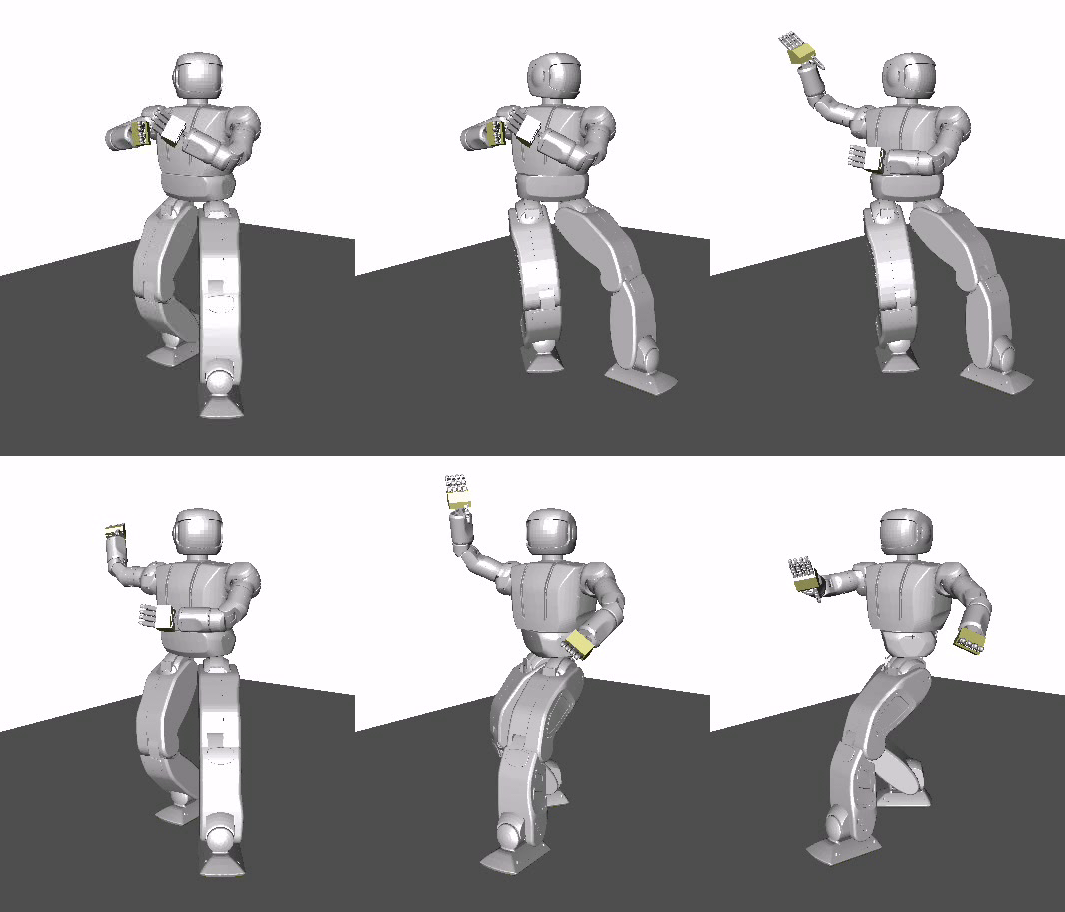
\includegraphics[width=1.0\columnwidth]{./pix/keyframe/keyframe.png}
  \caption{OpenHUBO using key-frame based method for throwing trajectory creation.  Frames are read from top left to bottom right.  Video of the above trajectory can be found at http://danlofaro.com/urai2012/\#keyframe}
  \label{fig:keyframe-throw}
\end{figure}

To ensure stability throughout the motion the balance controller as described in Section~\ref{sec:sec:balance} was applied and the static ZMP criteria was checked for the entire trajectory.
The resulting end effector velocity was 4.8 $\frac{m}{s}$ at the release point.  
Fig.~\ref{fig:keyframe-graph} shows the plot of the magnitude of the end effector's velocity.  
It should be noted that at the instance of release the velocity vector is at an elevation of $40^o$ from the ground.

\begin{figure}[t]
  \centering
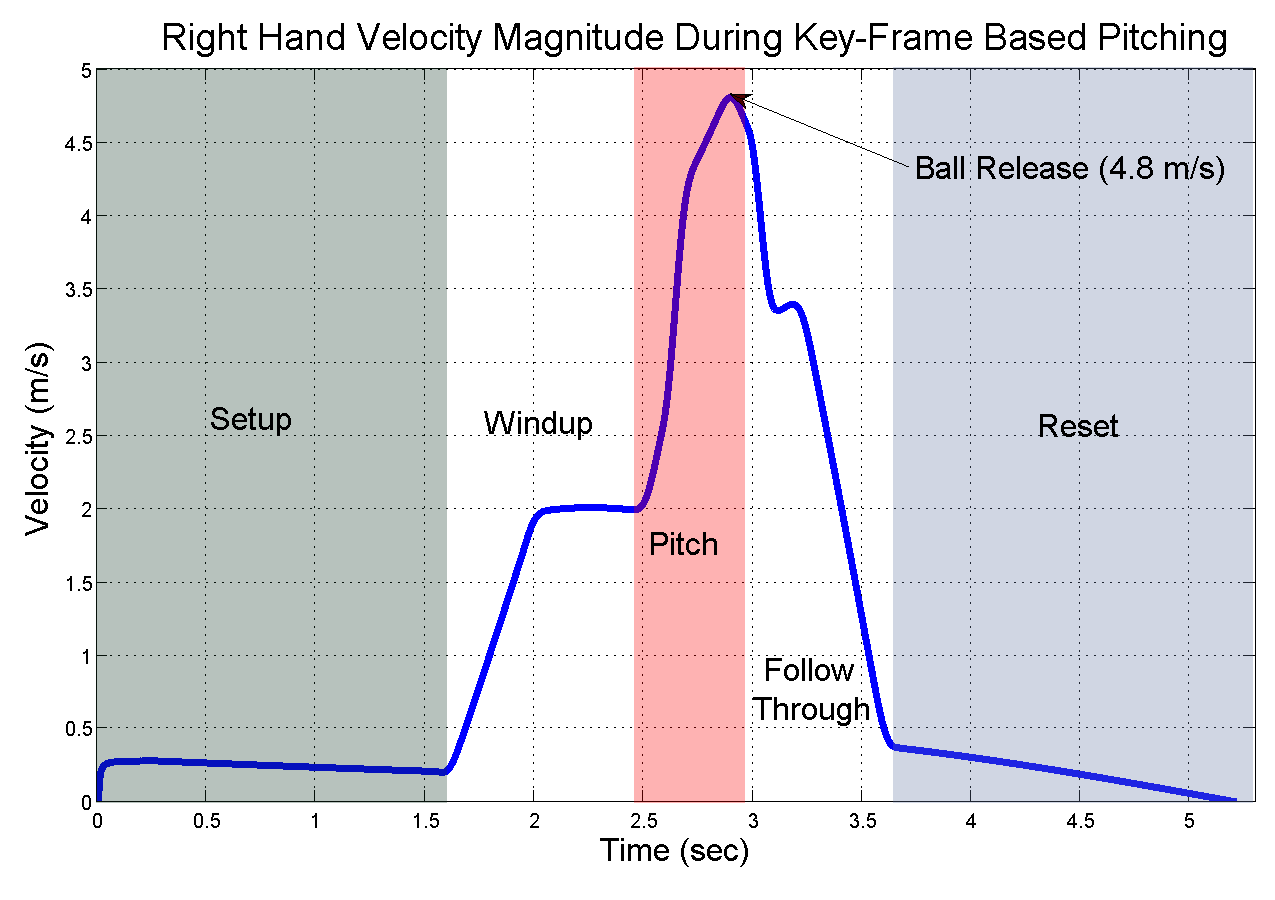
\includegraphics[width=1.0\columnwidth]{./fig/keyFrameThrow4.pdf}
  \caption{Velocity vs. Time graph showing the magnitude of the end-effector's velocity for the key-frame based throwing motion.  The six different stages of pitching are also shown.  Setup: move from the current position to th throw stance.  Windup: end effector starts to accelerate from the throw stance and move into position for the start of the pitch state. Pitch: end effector accelerates to release velocity.  Ball Release: the ball leaves the hand at maximum velocity (4.8 $\frac{m}{s}$) at an elevation of $40^o$ from the ground.  Follow Through: reducing velocity of end effector and all joints.  Reset: moves to a ready state for anther throw if needed.}
  \label{fig:keyframe-graph}
\end{figure}

\section{Method Comparison}\label{sec:comparison}
All three methods described are stable during the throwing motion and can successfully throw a baseball.  Table~\ref{table:comp} shows the end-effector (EEF) velocity, joint failure rate, overhand or underhand throwing and stability of the three different methods of end-effector velocity control used in this paper human-robot joint mapping (MoCap), SRM based and key-frame.

\begin{table}[!t]
%% increase table row spacing, adjust to taste
\renewcommand{\arraystretch}{1.3}
% if using array.sty, it might be a good idea to tweak the value of
% \extrarowheight as needed to properly center the text within the cells
\caption{Comparison between the three different methods of end-effector (EEF) velocity control: human-robot joint mapping (MoCap), SRM based and key-frame}
\label{table:comp}
\centering
\begin{tabular}{|c|c|c|c|c|}
\hline
  				& EEF 																	& Joint 						& Throw						& Stable  			\\
  				& Velocity ($\frac{m}{s}$)							& Failure (\%)			& Overhand (y/n)	& (y/n)					\\
\hline	
MoCap 		& 4.0																		& 0									& n								& y 						\\
\hline
SRM 			& 4.9																		& 10								& y								& y							\\
\hline
Key-Frame & 4.8 																	& 0 								& y								&	y							\\
\hline
\end{tabular}
\end{table}

The SRM technique worked well however the large jerk on each of the joints created large torques caused the motor controller to over torque/current and shutdown 10\% of the time.  
The pitch needs to work 100\% of the time thus this method is not well suited for the event.  
Both the human-robot joint mapping via MoCap and key-frame based methods consistently worked and stayed stable.  A secondary objective is to have the throwing motion be overhand like a standard Major League Baseball pitcher.  
Due to the constraints placed on the joint mapping of the MoCap method in Section~\ref{sec:sec:mocap} an over arm throw would be impossible to preform due to the robot's $\pm180^o$ joint limitations.  The key-frame method was chosen as the method to throw the ball.  
%Section~\ref{sec:finalDesign} describes the modifications to the system to allow it to reliably throw the pitch the desired distance.
\section{\bf Final Design}\label{sec:finalDesign}

The final goal is to have an end-effector velocity of 9.47 $\frac{m}{s}$ at $45^o$.  
The key-frame method was tested to throw at 4.8 $\frac{m}{s}$.  
To increase the end-effector velocity the upper body motion was kept unchanged but the lower body added a stepping motion with its legs.
The stepping motion consists of lifting the left foot up, pushing forward with the right and move the left forward 10 cm.  
Stepping with your non-dominant foot, and pushing with the dominant, when throwing overhand, is common practice to increase the distance you can throw a ball.  
Jaemi Hubo throws with its right hand and steps with its left.  
This increased the end-effector velocity from 4.8 $\frac{m}{s}$ to 7.1 $\frac{m}{s}$.
Fig.~\ref{fig:hubo-step} shows the stepping motion of the robot.

\begin{figure}[t]
  \centering
\includegraphics[width=1.0\columnwidth]{./pix/stepthrow.png}
  \caption{(Left) Hubo stepping 10 cm up and forwards while pushing with dominant foot.  (Right) Hubo lands with non-dominant foot. As a result the end effectors velocity is increased by 2.3 $\frac{m}{s}$.}
  \label{fig:hubo-step}
\end{figure}


The addition of pushing off with the right foot and stepping forward introduced two problems.  1) The ZMP criteria is not satisfied throughout the motion and 2) the right foot would slip when pushing its body forward.  
To avoid slip \textit{hook and loop} was paced on the bottom of the right foot (dominant) and on the throwing platform.  
This did not permanently attach the robot to the platform but it did allow for more friction between the foot and the ground.
This allowed the balancing controller to function adequately for the short step and maintain stability.
The platform was added to ensure a more consistent ground for the robot to balance on than the baseball field can inherently provide.


%\begin{figure*}[t]
%  \centering
%\includegraphics[width=1.0\textwidth]{./pix/preThrow2.png}
%  \caption{Frame overlay of the Hubo throwing overhand a distance of 10 m (32.8 feet) with a release angle of 40$^o$ and a tip speed of 10 $\frac{m}{s}$.  Captured at 20 fps with a shutter speed of 1/30 sec.  Each of the white dashes of in the image is the actual baseball as picked up by the video camera.}
%  \label{fig:hubo-throw-test}
%\end{figure*}

An additional 2.5 $\frac{m}{s}$ was needed to give a proper throw.  
Borrowing from the GRASP Lab and their high powered pneumatic wrist on their PhillieBot, a spring loaded mechanism was added to Hubo's wrist, see Fig.~\ref{fig:hubo-spring}.
The addition of this mechanism allowed the robot to achieve an end-effector velocity magnitude of 10 $\frac{m}{s}$.
Fig.~\ref{fig:hubo-throw-test} shows a frame overlay of the the Hubo throwing a regulation baseball 10 m (32.8 feet).
Fig.~\ref{fig:hubo-throw} shows the same throw at Citizens Bank Park on April $28^{th}$, 2012.






\section{Conclusion}\label{sec:conclusion}
The creation of a reliable humanoid throwing method was completed. 
This allowed the Hubo to complete its goal of becoming the first full-size humanoid to throw the first pitch at a Major League Baseball game.
Anthropomorphizing the robotic pitch was done via outfitting Jaemi with a uniform shirt and cap.
Hubo also gestured to the crowd via waving during its entrance and exit of the field to further engage the audience at the \textit{Science Night at the Ballpark}.
Three methods of creating a viable pitch were explored and tested: (1) human-robot mapping via motion capture, (2) sparse reachable map based trajectory generation and (3) a key-frame based method.  
Though the key-frame based method was the simplest it also proved to be the most viable.  
The balancing controller ensured stability of the system throughout the throw.  
The addition of a high powered wrist and having the robot step forward when it throws created conditions for a successful and reliable pitch.
The latter methods answered the challenges posed in the area of full-body locomotion, coordination and stabilization.

Prior full-size humanoid throwing methods such as the work by Kim et al. \cite{5686315,JooH2011438} were only shown in simulation.
This paper's set of experiments and demonstrations shows the realization of these same tasks in the physical world.
Throughout all of the experiments the system was manually aimed prior to each pitch.
Each of the robot's pitches are accurate however a key factor in off-target or \textit{wild} pitches is improper aiming during setup.
The addition of feedback via a targeting system similar to that of Hu et al.~\cite{5649335} would remove the need for manual targeting of the robot.
Feedback via a targeting system will be incorporated in the next revision.

This work is a step towards full-size humanoids performing fast and accurate full body tasks.
Though one might perceive robots to be \textit{better} than people (faster, more accurate, etc.) the reality is that the field of humanoid robotics is still in its infant state and Hubo is only the size of a ten year old child.
Having Hubo complete this task shows that full-size humanoids can perform some tasks at a ten year old's level.
More information and media about this event is available on this papers home page http://danlofaro.com/Humanoids2012/



%In in completing this challenge the overarching fields of fully  

%of full body locomotion/coordination and stability were addressed.









%The challenges in completing this task included full body locomotion, stabilization, 


% An example of a floating figure using the graphicx package.
% Note that \label must occur AFTER (or within) \caption.
% For figures, \caption should occur after the \includegraphics.
% Note that IEEEtran v1.7 and later has special internal code that
% is designed to preserve the operation of \label within \caption
% even when the captionsoff option is in effect. However, because
% of issues like this, it may be the safest practice to put all your
% \label just after \caption rather than within \caption{}.
%
% Reminder: the "draftcls" or "draftclsnofoot", not "draft", class
% option should be used if it is desired that the figures are to be
% displayed while in draft mode.
%
%\begin{figure}[!t]
%\centering
%\includegraphics[width=2.5in]{myfigure}
% where an .eps filename suffix will be assumed under latex, 
% and a .pdf suffix will be assumed for pdflatex; or what has been declared
% via \DeclareGraphicsExtensions.
%\caption{Simulation Results}
%\label{fig_sim}
%\end{figure}

% Note that IEEE typically puts floats only at the top, even when this
% results in a large percentage of a column being occupied by floats.


% An example of a double column floating figure using two subfigures.
% (The subfig.sty package must be loaded for this to work.)
% The subfigure \label commands are set within each subfloat command, the
% \label for the overall figure must come after \caption.
% \hfil must be used as a separator to get equal spacing.
% The subfigure.sty package works much the same way, except \subfigure is
% used instead of \subfloat.
%
%\begin{figure*}[!t]
%\centerline{\subfloat[Case I]\includegraphics[width=2.5in]{subfigcase1}%
%\label{fig_first_case}}
%\hfil
%\subfloat[Case II]{\includegraphics[width=2.5in]{subfigcase2}%
%\label{fig_second_case}}}
%\caption{Simulation results}
%\label{fig_sim}
%\end{figure*}
%
% Note that often IEEE papers with subfigures do not employ subfigure
% captions (using the optional argument to \subfloat), but instead will
% reference/describe all of them (a), (b), etc., within the main caption.


% An example of a floating table. Note that, for IEEE style tables, the 
% \caption command should come BEFORE the table. Table text will default to
% \footnotesize as IEEE normally uses this smaller font for tables.
% The \label must come after \caption as always.
%
%\begin{table}[!t]
%% increase table row spacing, adjust to taste
%\renewcommand{\arraystretch}{1.3}
% if using array.sty, it might be a good idea to tweak the value of
% \extrarowheight as needed to properly center the text within the cells
%\caption{An Example of a Table}
%\label{table_example}
%\centering
%% Some packages, such as MDW tools, offer better commands for making tables
%% than the plain LaTeX2e tabular whffich is used here.
%\begin{tabular}{|c||c|}
%\hline
%One & Two\\
%\hline
%Three & Four\\
%\hline
%\end{tabular}
%\end{table}


% Note that IEEE does not put floats in the very first column - or typically
% anywhere on the first page for that matter. Also, in-text middle ("here")
% positioning is not used. Most IEEE journals/conferences use top floats
% exclusively. Note that, LaTeX2e, unlike IEEE journals/conferences, places
% footnotes above bottom floats. This can be corrected via the \fnbelowfloat
% command of the stfloats package.







% conference papers do not normally have an appendix


% use section* for acknowledgement
\section*{Acknowledgment}

This project was conducted by the Drexel Autonomous Systems Lab (DASL), the Music Entertainment Technology Lab (MET)\footnote{Music Entertainment Technology Lab: http://music.ece.drexel.edu}, and sponsored by the National Science Foundation via the two grants; Partnerships for International Research and Education (\#0730206) and Major Research Infrastructure Recovery and Reinvestment (\#CNS-0960061).  Special thanks for organization and technical assistance goes to the Philadelphia Science Festival, Robert Ellenberg and Roy Gross.  The robot platform used was Hubo, designed and created by our partner Dr. Jun-Ho Oh, Department of Mechanical Engineering, Korean Advanced Institute of Science and Technology, Daejeon, South Korea.% <-this %





% trigger a \newpage just before the given reference
% number - used to balance the columns on the last page
% adjust value as needed - may need to be readjusted if
% the document is modified later
%\IEEEtriggeratref{8}
% The "triggered" command can be changed if desired:
%\IEEEtriggercmd{\enlargethispage{-5in}}

% references section

% can use a bibliography generated by BibTeX as a .bbl file
% BibTeX documentation can be easily obtained at:
% http://www.ctan.org/tex-archive/biblio/bibtex/contrib/doc/
% The IEEEtran BibTeX style support page is at:
% http://www.michaelshell.org/tex/ieeetran/bibtex/
%\bibliographystyle{IEEEtran}
% argument is your BibTeX string definitions and bibliography database(s)
%\bibliography{IEEEabrv,../bib/paper}
%
% <OR> manually copy in the resultant .bbl file
% set second argument of \begin to the number of references
% (used to reserve space for the reference number labels box)
%\begin{thebibliography}{1}

\bibliographystyle{IEEEtran}
%\bibliographystyle{plain}
\bibliography{throwing}{}
  
%\end{thebibliography}




% that's all folks
\end{document}


